\documentclass[10pt]{beamer}

\usepackage{xeCJK}
\setCJKmainfont{Noto Sans CJK SC}
\xeCJKsetup{PunctStyle=kaiming,CJKspace=true,CheckSingle=true} 

\DeclareGraphicsRule{*}{mps}{*}{}
\usepackage{subfigure}
\usepackage{amssymb, amsmath, amsfonts,verbatim}
\usepackage{tikz}
\graphicspath{ {./} }
\usetikzlibrary{matrix,arrows,fit,backgrounds,mindmap,plotmarks,decorations.pathreplacing}
\usepackage{tkz-euclide}
\usepackage{pgfplots}
\pgfplotsset{compat=1.12}
\pgfdeclarelayer{background}
\pgfsetlayers{background,main}

\tikzset{decoration={name=none},}

\newlength\figureheight
\newlength\figurewidth

\newcommand{\tikzdir}[1]{#1.tikz}
\newcommand{\inputtikz}[1]{\input{\tikzdir{#1}}}

\newcommand{\tI}{\tilde {\mathcal I}}
\newcommand{\tA}{\tilde A}
\newcommand{\ty}{\tilde y}
\newcommand{\tx}{\tilde x}
\newcommand{\tw}{\tilde w}
\newcommand{\tv}{\tilde v}
\newcommand{\tC}{\tilde C}
\newcommand{\tP}{\tilde P}
\newcommand{\Ic}{{\mathcal I^c}}
\newcommand{\J}{{\mathcal J}}
\newcommand{\K}{{\mathcal K}}

\newcommand{\diag}{\text{diag}}
\DeclareMathOperator{\1}{\textbf{1}}

\DeclareMathOperator{\Smin}{Smin}
\DeclareMathOperator{\Smid}{Smid}
\DeclareMathOperator{\Smax}{Smax}
\DeclareMathOperator{\MSE}{MSE}
\DeclareMathOperator{\rank}{rank}
\DeclareMathOperator{\Med}{Med}
\DeclareMathOperator{\Max}{Max}
\DeclareMathOperator{\Min}{Min}
\DeclareMathOperator{\tr}{tr}
\DeclareMathOperator{\Cov}{Cov}
\DeclareMathOperator{\logdet}{log\;det}
\DeclareMathOperator{\argmin}{arg\;min}
\DeclareMathOperator{\argmax}{arg\;max}
\let\Tiny\tiny

\DeclareMathOperator{\E}{\mathbb E}
\tikzstyle{sensor} = [draw, fill=blue!20, rectangle, rounded corners,
minimum height=2em, minimum width=7em]
\tikzstyle{est} = [draw, fill=orange!20, rectangle, rounded corners,
minimum height=2em, minimum width=7em]
\tikzstyle{pinstyle} = [pin edge={to-,thin,black}]


\title[Kalman Filter]{Kalman Filtering from 3 Different Perspectives}
\author[Yilin Mo]{Yilin Mo}
\institute[Tsinghua]{Department of Automation, Tsinghua University}
\date[May 12, 2021]{May 12, 2021}

\usetheme[block=fill]{metropolis}
\definecolor{thupurple}{RGB}{102,8,116}
\definecolor{caltechcolor}{RGB}{102,8,116}
\setbeamercolor{title separator}{fg=black!50}
\setbeamercolor{frametitle}{bg=thupurple!70!black}

\begin{document}

\begin{frame}
  \titlepage
\end{frame}

\frame{\tableofcontents}

\section{Introduction}
\begin{frame}{Motivation}
  \begin{itemize}
    \item Sensor Networks are becoming ubiquitous, with lots of interesting applications.
      \begin{itemize}
	\item environmental monitoring
	\item health care
	\item industrial monitoring
	\item military applications (threat detection)
      \end{itemize}
    \item {\bf Low cost} nodes with {\bf limited energy budget} and {\bf limited communication capability}.
    \item Communication is unreliable. 
    \item Communication costs too much resources (energy, bandwidth). 
    \item Sensor may be compromised.
    \item \ldots
    \item \bf How to do information fusion in sensor network?
  \end{itemize}
\end{frame}

\begin{frame}{LTI System}
  Consider the following LTI(Linear Time-Invariant) system:
  \begin{block}{System Description}
    \begin{displaymath}
      x_{k+1} = Ax_k +  w_k,\; y_{k} = C x_k + v_k.
    \end{displaymath}
  \end{block}
  \begin{itemize}
    \item $x_k \in \mathbb R^n$ is the state at time $k$.
    \item  $y_k \in \mathbb R^m$ is the measurements from the sensors. 
    \item $w_k,v_k,x_0$ are independent Gaussian random variables, and $x_0 \sim \mathcal N(\bar x,\;\Sigma)$, $w_k \sim \mathcal N(0,\;Q)$ and $v_k \sim \mathcal N(0,\;R)$. 
  \end{itemize}
\end{frame}

\begin{frame}{Kalman Filter}
  Define 
  \begin{displaymath}
    \begin{split}
      \hat x_k &\triangleq \E (x_k|y_k,\dots,y_0),\,e_k\triangleq  x_k -\hat x_k, \,P_k \triangleq \Cov(e_k).\\
      \hat x_k^- &\triangleq \E (x_k|y_{k-1},\dots,y_0),\,e_k^-\triangleq  x_k -\hat x_k^-, \,P_k^- \triangleq \Cov(e_k^-).
    \end{split}
  \end{displaymath}
  Kalman filter takes the following form:
  \begin{align*}
    Prediction:&&\\
	       &\hat x _{k + 1}^-  = A \hat x_{k} + Bu_k  , \quad P_{k + 1}^-  = AP_{k} A'  + Q ,\\
    Correction:&&\\
	       &\hat x_{k} = \hat x_{k}^-  + P_k^- C'(CP_k^- C'+R)^{-1} (y_k  - C \hat x _{k}^- ) , \\
	       &P_{k} = \left[(P_{k}^-)^{-1} + C' R^{-1} C \right]^{-1},
  \end{align*}
  with initial condition
  \begin{displaymath}
    \hat x_{0}^-  = \bar x_0 ,\quad P_{0}^-  = \Sigma.
  \end{displaymath}
\end{frame}

\begin{frame}{Kalman Filter}
  Define the following Lyapunov operator
  \begin{displaymath}
    h(X) \triangleq AXA'  + Q, 
  \end{displaymath}
  and Riccati operators
  \begin{displaymath}
    \tilde g(X) \triangleq (X^{-1} + C'R^{-1}C)^{-1},\,g \triangleq \tilde g\circ h.
  \end{displaymath}
  Hence,
  \begin{displaymath}
    P_{k+1}^- = h(P_k),\,P_{k+1} =\tilde g(P_{k+1}^-) =  g(P_k). 
  \end{displaymath}
\end{frame}

\begin{frame}{Properties of Kalman Filter}
  \begin{itemize}
    \item For KF, we need to keep track on both the state estimate $\hat x_k$ and the ``accuracy'' of the estimate $P_k$.
    \item $P_k$ is deterministic, which does not depends on $y_k$.
    \item If $(A,C)$ is detectable, $\{P_k\}$ is always bounded. In other words, the estimator is stable.
    \item If we further assume that $(A,Q^{1/2})$ is controllable, then $\{P_k\}$ converges to the unique solution of algebraic Riccati equation 
      \begin{displaymath}
	X = g(X). 
      \end{displaymath}
  \end{itemize}
\end{frame}

\section{Kalman Filter is a Bayes Filter for Linear Gaussian System}

\begin{frame}{Bayes Filter for Hidden Markov Model} 
  \begin{itemize}
    \item Hidden Markov Model:
  \begin{center}
    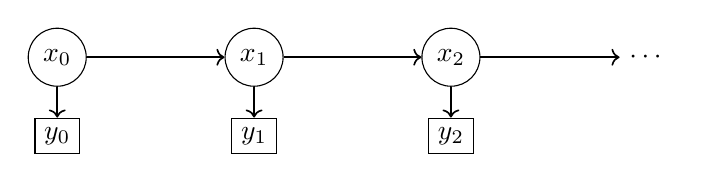
\begin{tikzpicture}[x=2.5cm, y=1cm]

      \node [circle, draw]     (x0)  at (0,0) {$ x_0$};
      \node [rectangle, draw]  (y10)  at (0,-1)   {$y_0$};
      \draw [<-,semithick,]  (y10) to (x0);

      \node  [circle, draw]          (x1)  at (1,0) {$ x_1$};
      \node [rectangle, draw]  (y11)  at (1,-1)   {$y_1$};
      \draw [<-,semithick,]  (y11) to (x1);

      \node  [circle, draw]          (x2)  at (2,0) {$ x_2$};
      \node [rectangle, draw]  (y12)  at (2,-1)   {$y_2$};
      \draw [<-,semithick,]  (y12) to (x2);

      \node           (x3)  at (3,0) {$ \cdots$};
      \draw [->,semithick] (x0) to (x1);
      \draw [->,semithick] (x1) to (x2);
      \draw [->,semithick] (x2) to (x3);
    \end{tikzpicture}
  \end{center}


    \item Bayes Filter:
      \begin{align*}
	Prediction:&&\\
		   &p(x_{k+1}|y_{0:k}) = \int p(x_{k+1}|x_{k})p(x_{k+1}|y_{0:k}) dx_k\\
	Correction:&&\\
		   &p(x_{k}|y_{0:k}) = \frac{ p(y_{k}|x_{k})p(x_{k}|y_{0:k-1})}{\int p(y_{k}|x_{k})p(x_{k}|y_{0:k-1}) dx_k}
      \end{align*}
    \item In general, need to keep track of the {\bf probability distribution}! 
    \item However, for linear Gaussian system, the distribution is always {\bf Gaussian} 
    \item Only need to track the {\bf mean and variance}
  \end{itemize}
\end{frame}
\subsection{Event-Based Sensor Scheduling}
\frame{\tableofcontents[currentsection]}
\begin{frame}{Sensor Scheduling}
  \begin{itemize}
    \item Communication costs too much energy
    \item Sensors could deliberately drop some packets to save energy
    \item Define the communication rate $r$ to be
      \begin{displaymath}
	r = \limsup_{k\rightarrow\infty}\frac{1}{N}\sum_{i=0}^{N-1}\gamma_i 
      \end{displaymath}
    \item Trade-off between energy consumption and estimation quality.
    \item When to send the information?
  \end{itemize}
\end{frame}

\begin{frame}{Sensor Scheduling: Off-line Schedule}
  The schedule is based on the statistics of the system, and hence can be determined off-line:
  \begin{itemize}
    \item Deterministic Schedule: send the temperature only at even time. 
    \item Stochastic Schedule: send the temperature with 50\% probability at each time. 
  \end{itemize}

  If no measurement arrives at time $k$, then the fusion center can only perform a prediction update.
\end{frame}

\begin{frame}{Sensor Scheduling: Event-Based Schedule}
  \begin{itemize}
    \item The schedule depends on both the statistics and the realization of the system. 
    \item Fox example, if the temperature of the room is normal distributed around $72.5$, we could design the schedule to be: send the temperature if the temperature is outside $[70,75]$.
    \item Even if no measurement arrives at time $k$, the fusion center can still perform a correction step, since it knows that the temperature is inside $[70,75]$.
  \end{itemize}
\end{frame}

\begin{frame}{Optimal Filter for Event-Based Schedule}

  \begin{itemize}
    \item When $\gamma_k = 0$, $y_k$ is a truncated Gaussian.
      \setlength\figureheight{2cm}
      \setlength\figurewidth{3cm}
      \begin{center}
	\inputtikz{gaussian}$\times$\inputtikz{det}$\Rightarrow$\inputtikz{det2}
      \end{center}
    \item The optimal filter is a Bayes filter 
    \item Need to keep track of the pdf of $x_k$ given $y_k,\dots,y_0$.
    \item Not linear in general, difficult to analyze the performance.
  \end{itemize}
\end{frame}

\begin{frame}{A Stochastic Event-Trigger}
  \setlength\figureheight{2cm}
  \setlength\figurewidth{3cm}
  \begin{center}
    \inputtikz{gaussian}$\times$\inputtikz{rand}$\Rightarrow$\inputtikz{rand2}
  \end{center}
  \begin{itemize}
    \item At each time $k$, the sensor generates a random variable $\zeta_k\sim U[0,1]$ .
    \item Decide whether to send or not based on the following rule:
      \begin{displaymath}
	\gamma_k= \begin{cases}
	  0&\zeta_k \leq \Phi(y_k)\\
	  1&\zeta_k > \Phi(y_k)
	\end{cases},
      \end{displaymath}
      where $\Phi$ is defined as
      \begin{displaymath}
	\Phi(y) = \exp\left( -\frac{1}{2}y'Yy \right). 
      \end{displaymath}
  \end{itemize}
\end{frame}

\begin{frame}{Optimal Filter}
  The optimal filter is similar to the KF:
  \begin{align*}
    Prediction:&&\\
	       &\hat x _{k + 1}^-  = A \hat x_{k} + Bu_k  , \quad P_{k + 1}^-  = h(P_k)\\
    Correction:&&\\
	       &\hat x_{k} = \begin{cases}
		 \hat x_{k}^-  + P_k^- C'(CP_k^- C'+R)^{-1} (y_k  - C \hat x _{k}^- ) & \gamma_ k = 1\\ 
		 (I - P_k^-C'(CP_k^-C'+R+Y^{-1})^{-1}C)\hat x_{k}^-   & \gamma_ k = 0 
	       \end{cases}\\
	       &P_{k} =\begin{cases}
		 \left[\left(P_k^-\right)^{-1} + C'\alert{R}^{-1}C\right]^{-1} & \gamma_k = 1\\
		 \left[\left(P_k^-\right)^{-1} + C'\left( \alert{R+Y^{-1} }\right)^{-1}C\right]^{-1}  &\gamma_k = 0
	       \end{cases}
  \end{align*}
  with initial condition
  \begin{displaymath}
    \hat x_{0}^-  = \bar x_0 ,\quad P_{0}^-  = \Sigma.
  \end{displaymath}
\end{frame}

%  \begin{frame}{Communication Rate}
%    \begin{theorem}
%      Let $\Pi_k = \Cov(y_k)$, then
%      \begin{displaymath}
%	P(\gamma_k = 1) = 1-1/\sqrt{\det(I+\Pi_kY)}.
%      \end{displaymath}
%      If the system is stable, then $\Pi_k\rightarrow \Pi$, which is given by
%      \begin{displaymath}
%	\Pi = CX C' + R,
%      \end{displaymath}
%      where $X = \lim_k \Cov(x_k)$ is the solution of the following Riccati equation
%      \begin{displaymath}
%	X = AXA' + Q. 
%      \end{displaymath}
%      The communication rate satisfies
%      \begin{displaymath}
%	r = 1-\frac{1}{\sqrt{\det(I+\Pi Y)}}.
%      \end{displaymath}
%    \end{theorem}
%  \end{frame}
%
%
%  \begin{frame}{Estimation Performance}
%    \begin{itemize}
%      \item When no packet arrives, it is equivalent to using a sensor with noise covariance $R + Y^{-1}$.
%      \item $P_k$ is always bounded even if no packet arrives. 
%      \item $P_k$ is oscillating between $\underline P$ and $\overline P$, which are the solution of the following Riccati equations:
%	\begin{displaymath}
%	  \begin{split}
%	    \overline P &= \left[\left(A\overline PA' + Q\right)^{-1} + C'\left( \alert{R+Y^{-1} }\right)^{-1}C\right]^{-1}\\
%	    \underline P &= \left[\left(A\underline PA' + Q\right)^{-1} + C'\alert{R}^{-1}C\right]^{-1}.
%	  \end{split}
%	\end{displaymath}
%      \item Using the concavity and monotonicity of Riccati equation, a lower bound of $\E P_k$ can be derived as the solution of the following Riccati equation:
%	\begin{displaymath}
%	    P= \left[\left(A PA' + Q\right)^{-1} + C' \alert{R_1}^{-1}C\right]^{-1},
%	\end{displaymath}
%	where
%	\begin{displaymath}
%	  R_1 = \left( rR^{-1} + (1-r)(R+Y^{-1})^{-1} \right)^{-1}.
%	\end{displaymath}<++>
%    \end{itemize}
%  \end{frame}
%
%  \begin{frame}{Event-Trigger Parameter Optimization}
%    We consider the following optimization problem:
%    \begin{align*}
%      &\mathop{\textrm{minimize}}\limits_{Y}&
%      & r\nonumber\\
%      &\textrm{subject to}&
%      & \overline P\leq \Delta.
%    \end{align*}
%    Using matrix inversion lemma, the constraint can be rewritten in SDP form as:
%    \begin{align*}
%      \left[ {\begin{array}{*{5}c}
%	Q^{-1}-M_1  &  Q^{-1}A\\
%	A^{\prime}Q^{-1} & A^{\prime}Q^{-1}A + S
%      \end{array}} \right] &\ge 0 \nonumber
%      \\
%      \left[ {\begin{array}{*{5}c}
%	R^{-1}-M_2  &  R^{-1}\\
%	R^{-1} & R^{-1}+Y
%      \end{array}} \right] &\ge 0 \nonumber
%      \\ M_1 - S + C^{\prime}M_2C &\ge 0 \nonumber \\
%      Y \ge 0, ~ S &\ge \Delta^{-1}
%    \end{align*}
%  \end{frame}
%
%  \begin{frame}{Event-Trigger Parameter Optimization}
%    The communication rate $r$ can be bounded by
%    \begin{displaymath}
%      1-\frac{1}{\sqrt{1+\tr(\Pi Y)}} \leq  r \leq 1-\exp\left(-\frac{1}{2}\tr(\Pi Y)\right).
%    \end{displaymath}
%    The optimization problem can be relaxed to
%    \begin{align*}
%      &\mathop{\textrm{minimize}}\limits_{Y}&
%      & \tr(\Pi Y)\nonumber\\
%      &\textrm{subject to}&
%      & \overline P\leq \Delta.
%    \end{align*}
%    If the optimal $Y$ of the relaxed problem is rank $1$, then it is also optimal for the original problem.
%  \end{frame}

\begin{frame}{Numerical Examples}
  We consider the following system
  \begin{displaymath}
    A = 0.8,\,C = 1,\, Q = R = 1. 
  \end{displaymath}
  \setlength\figureheight{5cm}
  \setlength\figurewidth{8cm}
  \begin{center}
    \inputtikz{eventbased}
  \end{center}
\end{frame}


\section{Kalman Filter is Solving a Least Square Problem}

\begin{frame}{Maximum a posteriori Estimator}
  \begin{itemize}
    \item Consider a Gaussian state $x\in \mathbb R^n$:
      \begin{displaymath}
	\E x = \bar x,\,\Cov(x) = \E xx^T = \Sigma.
      \end{displaymath}
    \item Let $y\in\mathbb R^m$ be our observation of $x$, which satisfies:
      \begin{displaymath}
	y = C x + v,
      \end{displaymath}
      where $v\sim \mathcal N(0,R)$ is a Gaussian measurement noise. 
    \item Given the measurement $y$, the MAP estimate $\hat x$ is a linear estimator:
      \begin{align*}
	\hat x &= \argmax_x {p(y|x)}\\
	       &= \argmin_x (y-Cx)'R^{-1}(y-Cx) + (x-\bar x)'\Sigma^{-1} (x-\bar x)\\
	&= \bar x + \Sigma C'(C\Sigma C'+R)^{-1}(y-C\bar x).
      \end{align*}
    \item The error $e = x - \hat x$ is zero mean Gaussian and
      \begin{displaymath}
	\Cov(e) = (\Sigma^{-1} +  C'  R^{-1}C)^{-1}.
      \end{displaymath}
  \end{itemize}
\end{frame}


\begin{frame}{MAP Estimator for LTI System}
  \begin{itemize}
    \item Suppose at time $k$, we want to estimate the current state $x_k$.
    \item We have available the current and the past observations $y_k,y_{k-1},\dots,y_0$.
    \item We could write down the relationship between $y_k,\dots,y_0$ and $x_k$ as follows:
      \begin{displaymath}
	\begin{split}
	  y_k& = C x_k + v_k \\
	  y_{k-1} & = Cx_{k-1}+v_{k-1} = CA^{-1}x_k -C A^{-1}w_{k-1} + v_{k-1}\\
		  &\vdots
	\end{split}
      \end{displaymath}
    \item Conceptually, one could use the MAP estimator to derive $\hat x_k$.
    \item Kalman filter is a recursive and efficient way of computing such problem 
  \end{itemize}
\end{frame}

\subsection{Kalman Filtering with Intermittent Observations}
\frame{\tableofcontents[currentsection]}

\begin{frame}{Classical Kalman Filter in Unreliable Network}
  Kalman filter assumes that all the observations $y_0,y_1,\ldots,y_k$ are available at time $k$.

  However in an unreliable network, observation packets can be lost, corrupted or significantly delayed.
  \begin{figure}[<h>]
    \begin{center}
      \includegraphics{slides.2}
    \end{center}
  \end{figure}
  What is the form of optimal Filter? 
\end{frame}

\begin{frame}{Channel Models}  
  \begin{itemize}
    \item Erasure channel: The estimator does not use corrupted or significantly delayed packets (treated as lost). 
    \item Single sensor: All the measurements made at time $k$ are contained in a single packet and hence it is either received in full or lost completely.
      \[
	\widetilde y_k = \gamma_k y_k,\;\gamma_k=0,1
      \]
    \item Memoryless channel: $\gamma_i$s are i.i.d. distributed and $P(\gamma = 1) = p$.
  \end{itemize}
\end{frame}

\begin{frame}{Kalman Filter with Intermittent Observation}
  (Sinopoli, 04) This problem can still be solved recursively in a similar way as classical Kalman filter. 
  \begin{align*}
    Prediction:&&\\
	       &\hat x _{k + 1}^-  = A \hat x_{k} + Bu_k  , \quad P_{k + 1}^-  = h(P_k)\\
    Correction:&&\\
	       &\hat x_{k} = \begin{cases}
		 \hat x_{k}^-  + P_k^- C'(CP_k^- C'+R)^{-1} (y_k  - C \hat x _{k}^- ) & \gamma_ k = 1\\ 
		 \hat x_{k}^-   & \gamma_ k = 0 
	       \end{cases}\\
	       &P_{k} =\begin{cases}
		 \tilde g(P_k^-) & \gamma_k = 1\\
		 P_k^-&\gamma_k = 0
	       \end{cases}
  \end{align*}
  with initial condition
  \begin{displaymath}
    \hat x_{0}^-  = \bar x_0 ,\quad P_{0}^-  = \Sigma.
  \end{displaymath}
  What about performance?

\end{frame}

\begin{frame}{Kalman Filter with Intermittent Observation: Performance}
  $P_k$ satisfies the following equation:
  \begin{equation}
    P_{k+1}= \gamma_k g(P_k) + (1-\gamma_k) h(P_k).
    \label{eq:basicricattieqn}
  \end{equation}
  $P_k$ is now stochastic. 
  \begin{itemize}
    \item (Censi, 11; Kar, 12) Under mild assumptions, $P_k$ converges to a limit distribution.
    \item However, very strong assumptions are needed to compute the exact distribution 
      \begin{itemize}
	\item (Censi, 09) Non-overlapping condition: $h(X_1)\geq g(X_2)$, for all $X_1,X_2$.
	\item (Vakili, 09) $C$ is time-varying and random.
      \end{itemize}
    \item What about $\E P_k$?
  \end{itemize}
\end{frame}

\begin{frame}{Existence of Critical Value}
  \begin{displaymath}
    \begin{split}
      \E P_k &= \E\left[\gamma_k g(P_k) + (1-\gamma_k) h(P_k)\right]= p\alert{\E g(P_k)} + (1-p) h(\E P_k).
    \end{split}
  \end{displaymath}
  It is impossible to get a recursive equation of $\E P_k$ due to the non-linear nature of Riccati Equation. 

  An even simpler question: whether $\{\E P_k\}$ is uniformly bounded or not?
  \begin{theorem}
    (Sinopoli,04) Under i.i.d. packets loss, if $(A,Q^{\frac{1}{2}})$ is controllable, $(C,A)$ is detectable, and $A$ is unstable, then there exists a $p_c\in[0,1)$ such that
    \begin{eqnarray}\label{eqn:lambdaCrit}
      \lim_{k\rightarrow\infty}\E P_k=+\infty & \mbox{for } 0\leq
      p \leq p_c \; \;
      \mbox{and  \hspace{3mm}$\exists P_0 \geq 0$}&\\
      \E P_k \leq M_{P_0} \;\; \forall k & \mbox{for } p_c <
      p \leq 1 \; \; \mbox{and \hspace{3mm}$\forall P_0 \geq 0$}&
    \end{eqnarray}
    where $M_{P_0} > 0 $  depends on the initial condition $P_0 \geq 0$
  \end{theorem}
\end{frame}

\begin{frame}{Lower-Bound for the Critical Value}
  \begin{theorem}
    (Sinopoli,04) The lower bound of $p_c$ is given by
    \begin{displaymath}
      p_c \geq 1-\frac{1}{\rho^2}, 
    \end{displaymath}
    where $\rho$ is the spectral radius of $A$. Furthermore, if $C$ is full column rank, then the equality holds.
  \end{theorem}
  We call a system to be one-step observable if $C$ is full column rank.

  The one-step observability condition can be relaxed to
  \begin{itemize}
    \item (Sinopoli,04) $A$ only has one unstable eigenvalue;
    \item (Plarre,09) $C$ invertible on the observable subspace.
  \end{itemize}
  Roughly speaking, all these conditions imply that $g$ is bounded.
\end{frame}

\begin{frame}{A Counter Example where the Lower Bound is not Tight}

  Consider the following LTI system:
  \begin{displaymath}
    \begin{split}
      \left[ {\begin{array}{*{20}c}
	    x_{k+1,1}  \\
	    x_{k+1,2}
      \end{array}} \right] &=
      \left[ {\begin{array}{*{20}c}
	    0 & 2  \\
	    2 & 0 
	    \end{array}} \right]  \left[ {\begin{array}{*{20}c}
	    x_{k,1}  \\
	    x_{k,2}
      \end{array}} \right] + w_k,\\
      y_k &= \left[ {\begin{array}{*{20}c}
	    1 & 0 
      \end{array}} \right] x_k + v_k.
	  \end{split}
	\end{displaymath}
	\begin{center}
	  \includegraphics{pic.1}
	\end{center}
      \end{frame}

      \begin{frame}{A Least Square Formulation}
	\begin{itemize}
	  \item  Kalman filter solves the MAP problem recursive
	  \item The performance is related to a stochastic Riccati equation
	  \item Instead we can unwind the Kalman filter to consider MAP problem directly:
	\begin{displaymath}
	  \left[ {\begin{array}{*{20}c}
		{\gamma_k y_k } \\
		\vdots \\                                                           {\gamma_0y_0 } \\
		\bar x_0 \\
		\end{array}} \right] = \left[ {\begin{array}{*{20}c}                  
		{\gamma_k CA^{ - 1} } \\
		\vdots \\
		{\gamma_{0}CA^{ - k-1} } \\
		{A^{ - k - 1} } \\
	  \end{array}} \right]x_{k + 1} + noise.
	\end{displaymath} 
	\end{itemize}
      \end{frame}

      %
%      \begin{frame}{A Counter Example}
%	\begin{itemize} 
%	  \item $(A,C)$ is observable:
%	    \begin{displaymath}
%	      C = [1\;\;0],\,CA = [0\;\;2]; 
%	    \end{displaymath}
%	  \item However, $A^2 =4I$ and $(A^2,C)$ is not observable:
%	    \begin{displaymath}
%	      C = [1\;\;0],\,CA^2 = [4\;\;0]; 
%	    \end{displaymath}
%	  \item Half of the observations contains only contain ``redundant'' information.
%	  \item For a second-order system, let the eigenvalues of $A$ to be $\lambda_1$ and $\lambda_2$. If $|\lambda_1| = |\lambda_2|$ and the angle between $\lambda_1$ and $\lambda_2$ is $2\pi r/q$, then $A^q = const\times I$. Hence $(A^q,C)$ is not observable if $rank(C) = 1$.
%	  \item $1/q$ of the observations contains only contain ``redundant'' information.
%	\end{itemize}
%      \end{frame}
%
%      \begin{frame}{A Counter Example}
%	\begin{theorem}
%	  Consider the following unstable observable system:
%	  \begin{itemize}
%	    \item  $A$ is diagonalizable, $\rho = |\lambda_1| = |\lambda_2| $;
%	    \item  $rank(C) = 1$;
%	  \end{itemize}
%	  Let
%	  \begin{displaymath}
%	    \alpha = \frac{|\arg(\lambda_1)-\arg(\lambda_2)|}{2\pi}.	
%	  \end{displaymath}
%	  If $\alpha$ is irrational, then the critical value of the system is given by
%	  \begin{displaymath}
%	    p_c = 1-\frac{1}{\rho^2}.
%	  \end{displaymath}
%	  If $\alpha = r/q$ is rational, then the critical value is given by
%	  \begin{displaymath}
%	    p_c = 1-\frac{1}{\rho^{\frac{2}{1-1/q}}}.
%	  \end{displaymath}
%	\end{theorem}
%      \end{frame}
%
%      \begin{frame}{Non-Degeneracy}
%	\begin{itemize}
%	  \item One-step observability: reconstruct the state from $1$ measurements. Too strong. 
%	  \item Observability: reconstruct the state from $n$ sequential measurements. Too weak.
%	  \item Let $A = diag(\lambda_1,\ldots,\lambda_n)$, $C = [C_1,\ldots, C_n]$.
%	  \item Consider index set $\mathcal I = \{i_1,\ldots,i_l\}\subseteq \{1,\ldots,n\}$.
%	  \item Define $A_{\mathcal I} = diag(\lambda_{i_1},\ldots,\lambda_{i_l})$, $C_{\mathcal I} = [C_{i_1},\ldots,C_{i_l}]$.
%	  \item We call the subsystem $(A_{\mathcal I}, C_{\mathcal I})$ an equiblock if $\lambda_{i_1}=\ldots=\lambda_{i_l}$. 
%	  \item We call the subsystem $(A_{\mathcal I}, C_{\mathcal I})$ a quasi-equiblock if $|\lambda_{i_1}|=\ldots=|\lambda_{i_l}|$. 
%	    \begin{definition}
%	      A system is non-degenerate if $A$ is diagonalizable and every quasi-equiblock $(A_{\mathcal I},C_{\mathcal I})$ is one-step observable.
%	    \end{definition}
%	\end{itemize}
%      \end{frame}
%
%      \begin{frame}{Non-Degeneracy}
%	\begin{itemize}
%	  \item Consider the following system: 
%	    \begin{displaymath}
%	      \begin{split}
%		A = diag(2,2,3,-3), C = \left[ {\begin{array}{*{20}c}
%		      C_1,C_2,C_3,C_4
%		\end{array}} \right].
%	      \end{split}
%	    \end{displaymath}
%	  \item A system is observable if every equiblock is one-step observable: $C_1$, $C_2$ are linear independent.
%	  \item A system is non-degenerate if every quasi-equiblock is one-step observable: $C_1$, $C_2$ are linear independent and $C_3$, $C_4$ are linear independent.
%	  \item One-step observability implies that $C_1$, $C_2$, $C_3$, $C_4$ are linear independent.
%	  \item Non-degeneracy is stronger than observability, but weaker than one-step observability. 
%	\end{itemize}
%	\begin{theorem}
%	  If the system is non-degenerate, then $(A^k,C)$ is observable for any $k\in \mathbb N$. 
%	\end{theorem}
%      \end{frame}
%
      \begin{frame}{Critical Value and Tail Distribution for Non-Degenerate System}
	\begin{theorem}
	  For a system whose unstable part is non-degenerate, the critical value is the lower bound given by
	  \begin{displaymath}
	    p_c = 1-\frac{1}{\rho^2}.
	  \end{displaymath}
	  Furthermore, $P_k$ converges to a heavy-tailed distribution, i.e.,
	  \begin{displaymath}
	    \lim_k P(\tr(P_k)\geq M) \sim M^\varphi,
	  \end{displaymath}
	  where 
	  \begin{displaymath}
	    \varphi = \frac{\log(1-p)}{2\log \rho}.	
	  \end{displaymath}
	\end{theorem}
      \end{frame}

      \subsection{Privacy Preserving Consensus}

\frame{\tableofcontents[currentsection]}
      \begin{frame}{Centralized v.s. Distributed Algorithm}
	\begin{figure}[<+htpb+>]
	  \begin{center}
	    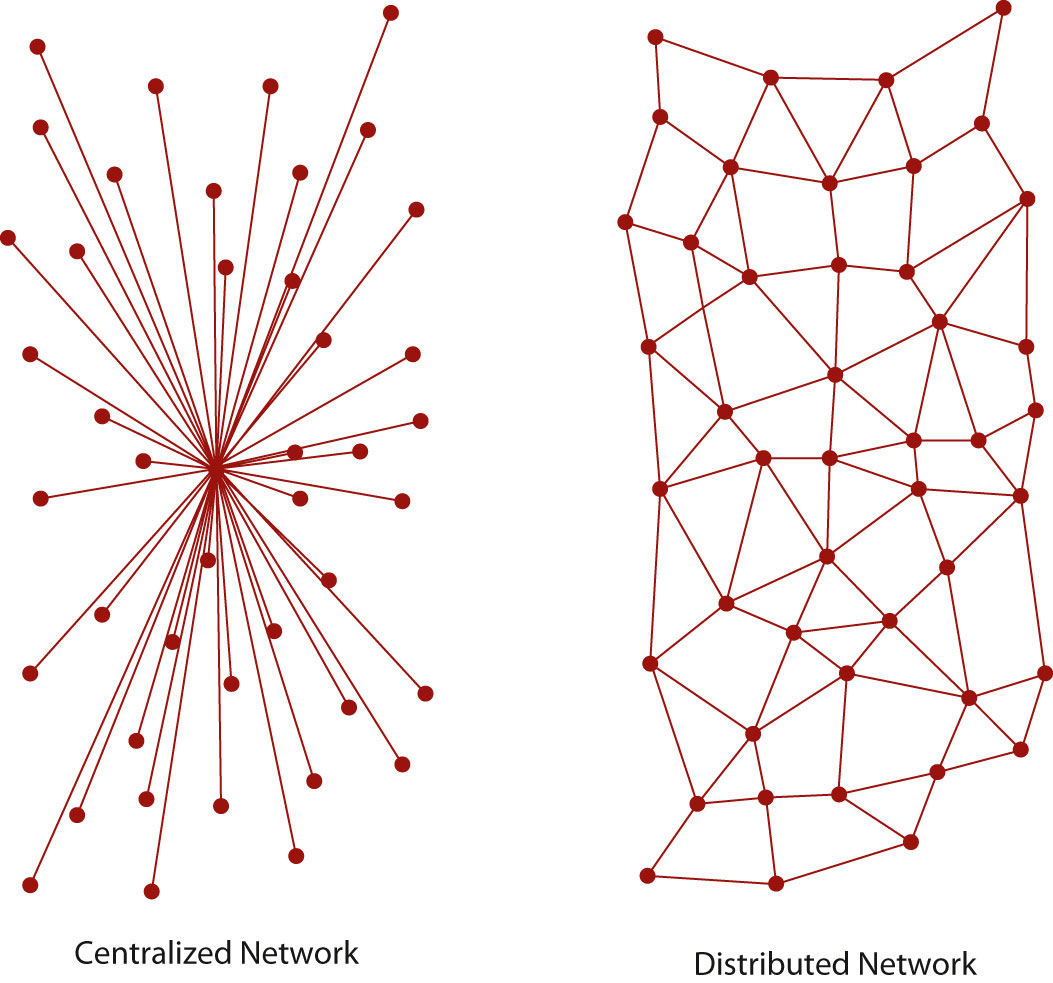
\includegraphics[width=0.50\textwidth]{centralized.png}
	  \end{center}
	\end{figure}
	Benefit of distributed algorithm: Reliability, Scalability, Transparency, Incremental Growth, Privacy
      \end{frame}

      \begin{frame}{Preliminary: Average Consensus}
	\begin{itemize}
	  \item We model the network composed of $n$ agents as an \emph{undirected} and \emph{connected} graph $G = \{V,\,E\}$.
	  \item Define the neighborhood of sensor $i$ as $\mathcal N(i)$.
	  \item Each agent has an initial scalar state $x_{i}(0)$.
	  \item Update equation:
	    \begin{displaymath}
	      x_i(k+1) = a_{ii} x_{i}(k) + \sum_{j\in \mathcal N(i)} a_{ij} x_{j}(k).  
	    \end{displaymath}
	  \item Update equation in matrix form:
	    \begin{displaymath}
	      x(k+1) = A x(k),
	    \end{displaymath}
	    where we assume that $A$ is \emph{symmetric}.
	\end{itemize}
      \end{frame}

      \begin{frame}{Preliminary: Average Consensus}
	Define the average vector as
	\begin{displaymath}
	  \bar x\triangleq \frac{\mathbf 1' x(0)}{n} \mathbf 1.
	\end{displaymath}
	The following conditions are necessary and sufficient for all the agents to reach average consensus:
	\begin{enumerate}
	  \item[(A1)] $ \lambda_1 = 1$ and  $|\lambda_i| < 1$ for all $i = 2,\ldots, n$.
	  \item[(A2)] $A\mathbf 1 = \mathbf 1$, i.e., $\mathbf 1$ is an eigenvector of $A$.
	\end{enumerate}
      \end{frame}

      \begin{frame}{Challenges}
	\begin{itemize}
	  \item Malicious Attacker: What if some agent do not follow the update rule:
	    \begin{displaymath}
	      x_i(k+1) = a_{ii} x_{i}(k) + \sum_{j\in \mathcal N(i)} a_{ij} x_{j}(k).  
	    \end{displaymath}

	    \emph{(Pasqualetti, Bicchi and Bullo, 2012)}: If there are $k$ malicious agents, then
	    \begin{itemize}
	      \item a benign node can detect the presence of malicious agents if the size of the minimum cut of the graph is at least $k + 1$.
	      \item a benign node can identify the set of the malicious agents if the size of the minimum cut of the graph is at least $2k + 1$.
	    \end{itemize} 

	  \item Curious Attacker: What if an agent wants to infer the initial state of other agents?
	  \item Malicious \& Curious Attacker?: Separation principle.
	\end{itemize}
      \end{frame}

      \begin{frame}{Privacy Concerns}
	\begin{itemize}
	  \item Without loss of generality, we consider agent $n$ wants to estimate the initial states of other agents.
	  \item Denote the neighborhood of agent $n$ as
	    \begin{displaymath}
	      \mathcal N(n) = \{j_1,\dots,j_m\}.
	    \end{displaymath}
	  \item Define
	    \begin{displaymath}
	      \begin{split}
		C &\triangleq \begin{bmatrix}
		  e_{j_1}&\dots&e_{j_m}&e_n
		\end{bmatrix}' \in \mathbb R^{(m+1)\times n},\\
		  y(k)&\triangleq \begin{bmatrix}x_{j_1}(k)&\dots&x_{j_m}(k)&x_n(k)
		  \end{bmatrix}=Cx(k).
		  \end{split}
		\end{displaymath}
	      \item The information set for agent $n$ at time $k$ is 
		\begin{displaymath}
		  \mathcal I(k) = \{y(0),\dots,y(k)\}. 
		\end{displaymath}
	    \end{itemize}
	  \end{frame}

	  \begin{frame}{Privacy Concerns}
	    For agent $n$, the problem becomes a standard estimation problem of the following linear system: 
	    \begin{displaymath}
	      x(k+1) = A x(k),\,y(k) = C x(k). 
	    \end{displaymath}
	    Since the system is noiseless, if $x_i$ is in the observable space of $(A,C)$, then agent $n$ can perfectly recover the initial state $x_i(0)$ of agent $i$. 

	    \alert{The privacy of agent $i$ is breached.}
	  \end{frame}

	  \begin{frame}{Example}
	    \begin{center}
	      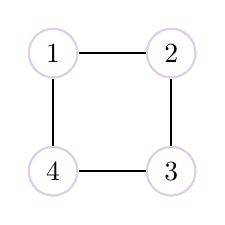
\begin{tikzpicture}
		\node (n4) at (0,0) [circle,draw=thupurple!50,draw=thupurple!20,thick] {4};
		\node (n1) at (0,1.5cm) [circle,draw=thupurple!50,draw=thupurple!20,thick] {1};
		\node (n3) at (1.5cm,0) [circle,draw=thupurple!50,draw=thupurple!20,thick] {3};
		\node (n2) at (1.5cm,1.5cm) [circle,draw=thupurple!50,draw=thupurple!20,thick] {2};
		\draw [semithick] (n1)--(n2)--(n3)--(n4)--(n1);
	      \end{tikzpicture}
	    \end{center}
	    \begin{enumerate}
	      \item At time step $0$, agent $4$ knows $x_1(0)$ and $x_3(0)$.
	      \item At time step $1$, agent $4$ knows $x_1(1)$, which is
		\begin{align*}
		  x_1(1) = a_{11}x_1(0)+a_{14}x_4(0)+a_{12}x_2(0).    
		\end{align*}
	    \end{enumerate}

	    For agent $4$, it can infer all the initial state $x(0)$ in two steps.

	  \end{frame}


	  \begin{frame}{Privacy Preserving Average Consensus}
	    \begin{enumerate}
	      \item At time $k$, each agent generates a standard normal distributed random variable $v_i(k)$ with mean $0$ and variance 1. We assume that all the random variables $\{v_i(k)\}_{i=1,\dots,n,\,k=0,1,\dots}$ are jointly independent.
	      \item Each agent then adds a random noise $w_i(k)$ to its state $x_i(k)$, where
		\begin{displaymath}
		  w_i(k) = \begin{cases}
		    v_i(0)&\text{, if }k = 0\\
		    \varphi^kv_i(k)-\varphi^{k-1}v_i(k-1)&\text{, otherwise}
		  \end{cases},
		  \label{eq:addednoise}
		\end{displaymath}
		where $0<|\varphi|<1$ is a constant for all agents. Define the new state to be $x_{i}^+(k)$, i.e.,
		\begin{displaymath}
		  x_{i}^+(k) = x_i(k) + w_i(k).  
		  \label{eq:noisestep}
		\end{displaymath}
	      \item Each agent then communicates with its neighbors and update its state to the average value, i.e.,
		\begin{displaymath}
		  x_i(k+1) = a_{ii}x_i^+(k)+\sum_{j\in \mathcal N(i)}a_{ij}x_{j}^+(k).
		  \label{eq:consensusstep}
		\end{displaymath}
	      \item There is no requirement for additional communication.
	    \end{enumerate}
	  \end{frame}

	  \begin{frame}{Privacy Preserving Average Consensus}
	    \begin{figure}[ht]
	      \begin{center}
		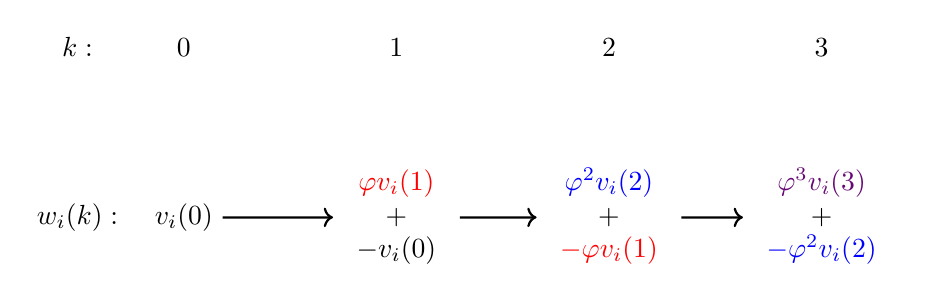
\begin{tikzpicture}[scale=0.9]
		  \node [label=above:$k:$] at (-1.5,0) {};
		  \node [label=above:$0$] at (0,0) {};
		  \node [label=above:$1$] at (3,0) {};
		  \node [label=above:$2$] at (6,0) {};
		  \node [label=above:$3$] at (9,0) {};
		  \node [] at (-1.5,-2) {$w_i(k):$};
		  \node [] (n0) at (0,-2){$v_i(0)$}; 
		  \node [] (n1) at (3,-2){$\begin{array}{c}\textcolor{red}{\varphi v_i(1)}\\+\\- v_i(0)\end{array}$}; 
		  \node [] (n2) at (6,-2){$\begin{array}{c}\textcolor{blue}{\varphi^2 v_i(2)}\\+\\\textcolor{red}{- \varphi v_i(1)}\end{array}$}; 
		  \node [] (n3) at (9,-2){$\begin{array}{c}\textcolor{thupurple}{\varphi^3 v_i(3)}\\+\\\textcolor{blue}{ -\varphi^2 v_i(2)}\end{array}$}; 
		  \draw [->,thick] (n0)--(n1);
		  \draw [->,thick] (n1)--(n2);
		  \draw [->,thick] (n2)--(n3);
		\end{tikzpicture}
	      \end{center}
	    \end{figure}
	  \end{frame}

	  \begin{frame}{Privacy Preserving Average Consensus}
	    \begin{itemize}
	      \item Update equation in matrix form:
		\begin{displaymath}
		  x(k+1) =Ax^+(k)= A(x(k) + w(k)).
		\end{displaymath}
	      \item Agent $n$ only receives a noisy version of the state:
		\begin{displaymath}
		  y(k) = C x^+(k) = C(x(k)+w(k)).	
		\end{displaymath}
	    \end{itemize}
	  \end{frame}

	  \begin{frame}{Performance Metric}
	    Define the error vector as
	    \begin{displaymath}
	      e(k) \triangleq x(k) - \bar x.
	    \end{displaymath}
	    Define the mean square convergence rate as
	    \begin{displaymath}
	      \rho \triangleq \limsup_{k\rightarrow\infty} \left( \sup_{z(0)\neq 0}\frac{\mathbb E_v e(k)'e(k)}{e(0)'e(0)}\right)^{1/k},
	    \end{displaymath}
	  \end{frame}

	  \begin{frame}{Performance Metric}
	    \begin{itemize}
	      \item The new information set of agent $n$ at time $k$ is
		\begin{displaymath}
		  \mathcal I(k) \triangleq \{x_n(0),y(0),\dots,y(k)\}.
		\end{displaymath}
	      \item Denote the maximum likelihood estimate of $x(0)$ given $\mathcal I(k)$ as $\hat x(0|k)$, the covariance of which is defined as $P(k)$.

	      \item  Clearly, $\mathcal I(k)\subset \mathcal I(k+1)$, which implies $P(k)\geq P(k+1)$. Hence, we can define

		\begin{displaymath}
		  P = \lim_{k\rightarrow\infty} P(k). 
		\end{displaymath}

		$P$ is best estimation performance that can be achieved by agent $n$ (with infinite observations).

	      \item If $P_{ii} = 0$, then agent $n$ can infer the initial state $x_i(0)$ of agent $i$ without any error (asymptotically).

	    \end{itemize}
	    Our goal is to make $\rho$ \emph{small}, while making $P$ \emph{large}.
	  \end{frame}

	  \begin{frame}{Convergence Result}
	    \begin{theorem}
	      For any initial condition $x(0)$, $x(k)$ converges to $\bar x$ in the mean square sense. Furthermore, the mean square convergence rate $\rho$ equals
	      \begin{displaymath}
		\rho = \max(|\varphi|^2,|\lambda_2|^2,|\lambda_n|^2).
	      \end{displaymath}
	    \end{theorem}
	    If we choose $\varphi$ to be small enough, then the added noise will not deteriorate the consensus speed.
	  \end{frame}

	  % \begin{frame}{Reduced System}
	  %   \begin{itemize}
	  %   \item Define $\tilde x(k) = \begin{bmatrix} x_1(k)&\dots&x_{n-1}(k) 
	  %     \end{bmatrix}$. 
	  %   \item $\tx(k)$ follows:
	  %     \begin{displaymath}
	  %       \tx(k+1) = \tA \tx^+(k) + \zeta x_n^+(k),
	  %     \end{displaymath}
	  %     where $\tA\in \mathbb R^{(n-1)\times(n-1)}$ is the principal minor of $A$ by removing the last row and column
	  %   \item Similarly, we can define
	  %     \begin{displaymath}
	  %       \ty = \begin{bmatrix}\tx^+_{j_1}(k)&\dots&\tx^+_{j_m}(k)
	  %       \end{bmatrix} = \tC \tx^+(k) .
	  %     \end{displaymath}
	  %   \item We assume that $(\tA,\tC)$ is observable, otherwise we can do a Kalman decomposition and only consider the observable space.
	  %   \end{itemize}
	  % \end{frame}
	  % 
	  % \begin{frame}{Reduced System}
	  %   \begin{theorem}
	  %     $\tilde A$ is strictly stable, i.e., $\|\tA\|<1$. 
	  %   \end{theorem}
	  %   \begin{itemize}
	  %   \item Consider the following $n-1$ by $n-1$ symmetric matrix
	  %     \begin{displaymath}
	  %       \mathcal S = (I-\tA)^{-1}\tC'\tC(I-\tA)^{-1}
	  %     \end{displaymath}
	  %   \item $I-\tA$ is invertible, $\tC$ is of rank $m$. Hence $\rank(\mathcal S) = m$. 
	  %   \item Let $\psi_1,\dots,\psi_{n-1}\in \mathbb R^{n-1}$ be the eigenvectors of $\mathcal S$. 
	  %   \item Assume that the eigenvalues corresponding to $\{\psi_1,\dots,\psi_m\}$ are non-zero and the eigenvalues corresponding to $\{\psi_{m+1},\dots,\psi_{n-1}\}$ are zero. 
	  %   \item Define
	  %     \begin{align}
	  %       \mathcal Q_1&\triangleq \begin{bmatrix}
	  %         \psi_1&\dots&\psi_m
	  %       \end{bmatrix}\in \mathbb R^{(n-1)\times m},\\
	  %       \mathcal Q_2& \triangleq \begin{bmatrix}
	  %         \psi_{m+1}&\dots&\psi_{n-1}
	  %       \end{bmatrix}\in \mathbb R^{(n-1)\times (n-m-1)}.
	  %     \end{align}
	  %   \end{itemize}
	  % \end{frame}

	  \begin{frame}{Estimation Performance}
	    \begin{itemize}
	      \item Measurement equation
	    \begin{displaymath}
	      y(k) =C\left( A^k x(0) + \sum_{t=0}^k A^{k-t}w(t)\right).
	    \end{displaymath}
	  \item Use Kalman-like filter to estimate $x(0)$ from $y(0),\ldots$
	    \end{itemize}
	    \begin{theorem}
	      Suppose that $0<\varphi<1$. $P$ is given by the following equality:
	      \begin{displaymath}
		P =\begin{bmatrix}
		  \mathcal Q_2\left[\mathcal Q_2'(I-\tA)^{-1}Y(I-\tA)^{-1}\mathcal Q_2\right]^{-1} \mathcal Q_2'&\mathbf 0\\
		  \mathbf 0'&0
		\end{bmatrix}
	      \end{displaymath}
	      where $ Y = \lim_{k\rightarrow\infty} Y(k)$ is the limit of the following recursive Riccati equations:
	      \begin{align*}
		Y(0)& = \tA \mathcal U \tA,\\
		Y(k+1) &=\tA \mathcal U\tA  +\varphi^{-2}\tA&\left[ Y^+(k) -  Y^+(k)\left(\varphi^2 I+Y^+(k) \right)^{-1}Y^+(k)\right]\tA,
	      \end{align*}
	      where
	      \begin{displaymath}
		Y^+(k) = \mathcal V Y(k) \mathcal V.
	      \end{displaymath}
	    \end{theorem}
	  \end{frame}

	  % \begin{frame}{Estimation Performance}
	  %   \begin{theorem}[Cont.]
	  %     Furthermore, the following inequalities hold:
	  %     \begin{displaymath}
	  %       \left( 1+\frac{\|\tA\|}{\varphi}\right)^{-2} \begin{bmatrix}
	  %         \Delta &\mathbf 0\\
	  %         \mathbf 0'&0
	  %       \end{bmatrix}\leq P \leq \left( 1-\frac{\|\tA\|}{\varphi}\right)^{-2} \begin{bmatrix}
	  %         \Delta &\mathbf 0\\
	  %         \mathbf 0'&0
	  %       \end{bmatrix}
	  %     \end{displaymath}
	  %     where
	  %     \begin{displaymath}
	  %       \Delta \triangleq \mathcal Q_2\left[\mathcal Q_2'(I-\tA)^{-1}\mathcal X(I-\tA)^{-1}\mathcal Q_2\right]^{-1} \mathcal Q_2',
	  %     \end{displaymath}
	  %     and $\mathcal X$ is the unique solution of the following Lyapunov equation
	  %     \begin{displaymath}
	  %       \mathcal X = \tA \mathcal X\tA /\varphi^2+  \tA\tC'\tC\tA . 
	  %     \end{displaymath}
	  %   \end{theorem}
	  % \end{frame}
	  \begin{frame}{Estimation Performance}
	    Define the essential neighborhood of sensor $i$ as 
	    \begin{displaymath}
	      \mathcal N_e(i) \triangleq \{j\in V:j\neq i,\,a_{ij}\neq 0\}.
	    \end{displaymath}
	    Node $j$ is called a super neighbor of $i$ if
	    \begin{enumerate}
	      \item $j$ is a neighbor of $i$.
	      \item $j$ is also a neighbor of all $i$'s essential neighbors.
	    \end{enumerate}

	    \begin{theorem}
	      The $i$th node's privacy is breached to node $j$ if and only if $j$ is a super neighbor of $i$.
	    \end{theorem}
	    The condition is can be checked \alert{locally}. In other words, your initial state can only be leaked to your neighbors.
	  \end{frame}
	  \begin{frame}{Estimation Performance}
	    \begin{center}
	      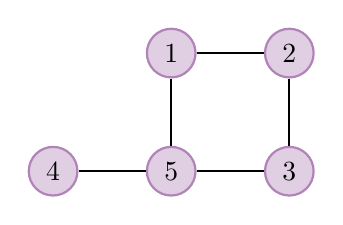
\begin{tikzpicture}
		\node (n4) at (-1.5cm,0) [circle,draw=thupurple!50,fill=thupurple!20,thick] {4};
		\node (n5) at (0,0) [circle,draw=thupurple!50,fill=thupurple!20,thick] {5};
		\node (n1) at (0,1.5cm) [circle,draw=thupurple!50,fill=thupurple!20,thick] {1};
		\node (n3) at (1.5cm,0) [circle,draw=thupurple!50,fill=thupurple!20,thick] {3};
		\node (n2) at (1.5cm,1.5cm) [circle,draw=thupurple!50,fill=thupurple!20,thick] {2};
		\draw [semithick] (n5)--(n1)--(n2)--(n3)--(n5)--(n4);
	      \end{tikzpicture}
	    \end{center}
	    \begin{displaymath}
	      \mathcal N(5)\bigcup \{5\} = \{1,3,4,5\}. 
	    \end{displaymath}
	    \begin{displaymath}
	      \mathcal N(4)\bigcup \{4\} = \{4,5\}. \text{ Agent 5 can perfectly infer }x_4(0).
	    \end{displaymath}
	    \begin{displaymath}
	      \mathcal N(1)\bigcup \{1\} = \{1,2,5\}.\text{ Agent 5 cannot perfectly infer }x_1(0)\text{ if }a_{12}\neq 0. 
	    \end{displaymath}
	  \end{frame}

	  % \begin{frame}{Estimation Performance}
	  %   \begin{center}
	  %     \begin{tikzpicture}
	  %       \node (n4) at (0,0) [circle,draw=caltechcolor!50,fill=caltechcolor!20,thick] {4};
	  %       \node (n1) at (0,1.5cm) [circle,draw=caltechcolor!50,fill=caltechcolor!20,thick] {1};
	  %       \node (n3) at (1.5cm,0) [circle,draw=caltechcolor!50,fill=caltechcolor!20,thick] {3};
	  %       \node (n2) at (1.5cm,1.5cm) [circle,draw=caltechcolor!50,fill=caltechcolor!20,thick] {2};
	  %       \draw [semithick] (n1)--(n2)--(n3)--(n4)--(n1);
	  %     \end{tikzpicture}
	  %   \end{center}
	  %   Assume $a_{ii} = a_{ij} = 1/3$, then agent $4$ can perfectly recover
	  %   \begin{displaymath}
	  %     x_4(0),\,x_1(0) + x_2(0) + x_3(0),\,x_1(0) - x_3(0).
	  %   \end{displaymath}
	  %   However, agent $4$ cannot infer $x_1(0)$, $x_2(0)$, $x_3(0)$ perfectly.
	  % \end{frame}
%
%	  \begin{frame}{Fundamental Limitation}
%	    \begin{itemize}
%	      \item If $P_{ii}=0$ using our average consensus algorithm, it is possible to design another noise sequence $\{w_i(k)\}$ to make $P_{ii}\neq 0$?
%
%	      \item Consider a more general noise model:
%		\begin{enumerate}
%		  \item $\mathbb Ew_i(k) = 0$.
%		  \item $\mathbb Ew_i(k_1)w_j(k_2) = 0$, when $i\neq j$.
%		\end{enumerate}
%	      \item The second condition implies that the sensors are not collaborating.
%	    \end{itemize}
%	  \end{frame}
%
%	  \begin{frame}{Fundamental Limitation}
%	    \begin{theorem}
%	      $x(k)$ converges to $\bar x$ in the mean squared sense, i.e.,
%	      \begin{displaymath}
%		\lim_{k\rightarrow\infty}\mathbb E  \,\|x(k)-\bar x\|^2 = 0,
%	      \end{displaymath}
%	      implies that for each agent $i$:
%	      \begin{displaymath}
%		\lim_{k\rightarrow\infty}\mathbb E \,\left(\sum_{t=0}^k w_i(t)\right)^2  = 0, \,\forall i=1,\dots,n.
%	      \end{displaymath}
%
%	    \end{theorem}
%	    Since the sensors are not collaborating, average consensus is achieved if and only if the noise from each sensor sums to 0 asymptotically (in the mean squared sense).
%	  \end{frame}
%
%	  \begin{frame}{Fundamental Limitation}
%	    \begin{theorem}
%	      Suppose that
%	      \begin{align*}
%		\lim_{k\rightarrow\infty}\mathbb E \,\left(\sum_{t=0}^k w_i(t)\right)^2  = 0, \,\forall i=1,\dots,n.
%	      \end{align*}
%	      Then $i$th node's privacy is breached to node $j$ \emph{if} $j$ is a super neighbor of $i$.
%	    \end{theorem}
%
%	    Comparing it to the previous theorem, we know that our proposed strategy achieves ``minimum'' privacy breach.
%	  \end{frame}

	  %% \subsection{Differential Privacy}
	  %% \begin{frame}{Differential Privacy}
	  %%   \begin{itemize}
	  %%   \item Denote the probability space generated by $\{v_i(k)\}$ as $(\Omega,\mathcal F,\mathbb P)$.
	  %%   \item Define $D = \mathbb R^n$ as the set of all possible initial condition $x(0)$.
	  %%   \item  Define a binary ``adjacency'' relation $\text{Adj}$ on $D$:
	  %%     \begin{displaymath}
	  %%       \text{Adj}(x^a(0),x^b(0)) \triangleq \begin{cases}
	  %%         1& \text{, if }\|x^a(0)-x^b(0)\|\leq d\\
	  %%         0&\text{, otherwise}
	  %%       \end{cases}.
	  %%     \end{displaymath}
	  %%   \item Let $\hat x_i(0|k)$ be the maximum likelihood estimate of the initial condition $x_i(0)$ of agent $i$ by agent $n$, given the information set $\mathcal I(k)$.
	  %%     \begin{align*}
	  %%       \hat x_i(0|k) = x_i(0) + \varsigma_i(k),	
	  %%     \end{align*}
	  %%     where $\varsigma_i(k)$ is a zero mean normal R.V. with variance $P_{ii}(k)\geq P_{ii}$.
	  %%   \item Clearly $\hat x_i(0|k)$ is a mapping from $D\times \Omega$ to $\mathbb R$, which can be written as
	  %%     \begin{displaymath}
	  %%       \hat x_i(0|k) = M_{i,k}(x(0),\,\omega),\,\text{where }x(0)\in D,\,\omega\in \Omega.
	  %%     \end{displaymath}
	  %%   \end{itemize}
	  %% \end{frame}
	  %% 
	  %% \begin{frame}{Differential Privacy}
	  %%   \begin{definition}
	  %%     The mapping $M_{i,k}$ is called $(\varepsilon,\delta)$-differentially private for $\text{Adj}$ if for all Borel-measureable $S\subseteq\mathbb R$ and adjacent initial conditions $x^a(0),x^b(0)$, the following inequality holds:
	  %%     \begin{displaymath}
	  %%       \mathbb P(M_{i,k}(x^a(0),\omega)\in S) \leq e^\varepsilon \mathbb P(M_{i,k}(x^b(0),\omega)\in S) +\delta.
	  %%     \end{displaymath}
	  %%   \end{definition}
	  %% \end{frame}

	  %% \begin{frame}{Relation with Differential Privacy}
	  %%   \begin{theorem}
	  %%     If $\varepsilon>0,0.5>\delta>0$ and
	  %%     \begin{displaymath}
	  %%       \frac{d}{2\varepsilon}(K + \sqrt{K^2+2\varepsilon})\leq P_{ii}, 
	  %%       \label{eq:epsilondelta}
	  %     \end{displaymath}
	  %     where $K =  Q^{-1}(\delta)$ and 
	  %     \begin{displaymath}
	  %       Q(x) \triangleq \frac{1}{\sqrt{2\pi}}\int_x^\infty \exp\left(-\frac{u^2}{2}\right)du,
	  %     \end{displaymath}
	  %     then for any $k\geq 0$, the mapping $M_{i,k}$ is $(\varepsilon,\delta)$-differentially private for $\text{Adj}$. 
	  %     \label{theorem:diffprivate}
	  %   \end{theorem}
	  % \end{frame}

	  \begin{frame}{Numerical Example}
	    \begin{center}
	      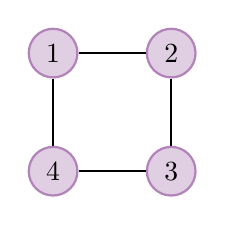
\begin{tikzpicture}
		\node (n4) at (0,0) [circle,draw=thupurple!50,fill=thupurple!20,thick] {4};
		\node (n1) at (0,1.5cm) [circle,draw=thupurple!50,fill=thupurple!20,thick] {1};
		\node (n3) at (1.5cm,0) [circle,draw=thupurple!50,fill=thupurple!20,thick] {3};
		\node (n2) at (1.5cm,1.5cm) [circle,draw=thupurple!50,fill=thupurple!20,thick] {2};
		\draw [semithick] (n1)--(n2)--(n3)--(n4)--(n1);
	      \end{tikzpicture}
	    \end{center}
	    \begin{itemize}
	      \item $a_{ii} = a_{ij} = 1/3$, for $j \in \mathcal N(i)$.
	      \item We choose $\varphi = 0.9$.
	    \end{itemize}
	  \end{frame}

	  \begin{frame}{Numerical Example: Convergence Result}
	    \begin{figure}[ht]
	      \begin{center}
		\setlength{\figureheight}{5cm}
		\setlength{\figurewidth}{6cm}
		\inputtikz{convergence}
	      \end{center}
	    \end{figure}
	  \end{frame}

	  \begin{frame}{Numerical Example:Estimation Performance}
	    \begin{figure}[ht]
	      \begin{center}
		\setlength{\figureheight}{5cm}
		\setlength{\figurewidth}{6cm}
		\inputtikz{variance}
	      \end{center}
	      \label{fig:variance}
	    \end{figure}
	  \end{frame}

	  % \section{Conclusion}
	  % \begin{frame}{Conclusion}
	  %   \begin{itemize}
	  %   \item We propose a privacy preserving average consensus algorithm.
	  %   \item We compute the exact mean square convergence rate of the proposed algorithm.
	  %   \item We derive the asymptotic estimation performance.
	  %   \item We provide a topological necessary and sufficient condition, under which the privacy of an agent is breached. 
	  %   \item We prove that our algorithm achieves minimum privacy breach, under the non-collaborating assumption.
	  %   \item We prove that our consensus algorithm is differentially private given that $P_{ii}\neq 0$. 
	  %   \end{itemize}
	  %   
	  % \end{frame}


	  % \begin{frame}{CPS Architecture}
	  %   \begin{center}
	  %     \begin{tikzpicture}[>=latex]
	  %       \draw [draw=caltechcolor!50,fill=caltechcolor!20,thick] (-4,-0.5) rectangle (4,0.5);
	  %       \node at (0,0) {Physical System};
	  %       \draw [draw=blue!50,fill=blue!20,thick] (-4,1.5) rectangle (4,2.5);
	  %       \node at (0,2) {Cyber Infrastructure};
	  %       \draw [draw=red!50,fill=red!20,thick] (-4,3.5) rectangle (4,4.5);
	  %       \node at (0,4) {Decision Making and Control};
	  %       \node [anchor=west] at (2,3) {Raw Data};
	  %       \node [anchor=east] at (-2,3) {Control};
	  %       \draw [thick,->] (-2,3.5)--(-2,2.5);
	  %       \draw [thick,->] (-2,1.5)--(-2,0.5);
	  %       \draw [thick,<-] (2,3.5)--(2,2.5);
	  %       \draw [thick,<-] (2,1.5)--(2,0.5);
	  %     \end{tikzpicture}
	  %   \end{center}
	  % \end{frame}
	  % 
	  % \begin{frame}{A Secure CPS Architecture}
	  %   \begin{center}
	  %     \begin{tikzpicture}[>=latex]
	  %       \draw [draw=caltechcolor!50,fill=caltechcolor!20,thick] (-4,-0.5) rectangle (4,0.5);
	  %       \node at (0,0) {Physical System};
	  %       \draw [draw=blue!50,fill=blue!20,thick] (-4,1.5) rectangle (4,2.5);
	  %       \node at (0,2) {Cyber Infrastructure};
	  %       \draw [draw=green!50,fill=green!20,thick] (-4,3.5) rectangle (4,4.5);
	  %       \node at (0,4) {Security Layer};
	  %       \draw [draw=red!50,fill=red!20,thick] (-4,5.5) rectangle (4,6.5);
	  %       \node at (0,6) {Decision Making and Control};
	  %       \node [anchor=west] at (2,3) {Raw Data};
	  %       \node [anchor=west] at (2,5) {Secured Data};
	  %       \node [anchor=east] at (-2,3) {Modified Control};
	  %       \node [anchor=east] at (-2,5) {Control};
	  %       \draw [thick,->] (-2,5.5)--(-2,4.5);
	  %       \draw [thick,->] (-2,3.5)--(-2,2.5);
	  %       \draw [thick,->] (-2,1.5)--(-2,0.5);
	  %       \draw [thick,<-] (2,5.5)--(2,4.5);
	  %       \draw [thick,<-] (2,3.5)--(2,2.5);
	  %       \draw [thick,<-] (2,1.5)--(2,0.5);
	  %     \end{tikzpicture}
	  %   \end{center}
	  % \end{frame}


	  \section{(Steady State) Kalman Filter is an LTI System with Multiple Inputs}

	  \subsection{Distributed Estimation}
	  \begin{frame}{Problem formulation}
	    \begin{itemize}
	      \item The system and measurement equation:
		\begin{align*}
		  x(k+1)&=Ax(k)+w(k)\\
		  y_i(k)&=C_ix(k)+v_i(k), \;\forall i\in\{1,...,m\}.
		\end{align*}
	    \end{itemize}
	  \end{frame}

	  \begin{frame}{Centralized Kalman filter}
	    \begin{itemize}
	      \item The centralized Kalman filter in steady state:
		\begin{align*}
		  \hat x(k+1)=(A-KCA)\hat x(k)+Ky(k+1),
		\end{align*}
	      \item Information flow:
		\begin{figure}
		  \centering
		  \resizebox{0.5\textwidth}{!}{\input{Kalman.tikz}}
		  %\caption{The information flow of centralized Kalman filter.}
		\end{figure}
	    \end{itemize}
	  \end{frame}

	  \begin{frame}{Distributed estimation: literature review}
	    \begin{itemize}
	      \item Sequential: require special communication topology which should be sequentially connected as a ring/chain.
	      \item Gossip: the sensor selects one node in its neighborhood, with which its local information is fused.
	      \item Consensus: perform the average consensus on local estimates, noisy measurements, ... 
	      \item etc...
	    \end{itemize}
	    {\scriptsize [1] B. Chen, G. Hu, D. W. Ho, and L. Yu, ``Distributed kalman filtering
	      for time-varying discrete sequential systems,” Automatica, vol. 99, pp.
	      228–236, 2019.

	      [2] K. Ma, S. Wu, Y. Wei, and W. Zhang, ``Gossip-based distributed tracking
	      in networks of heterogeneous agents,” IEEE Communications Letters,
	      vol. 21, no. 4, pp. 801–804, 2016.

	      [3] R. Olfati-Saber, ``Distributed kalman filtering for sensor networks,” in
	      2007 46th IEEE Conference on Decision and Control. IEEE, 2007, pp.
	      5492–5498.

	      [4] R. Olfati-Saber, ``Distributed kalman filter with embedded consensus filters,” in
	      Proceedings of the 44th IEEE Conference on Decision and Control.
	      IEEE, 2005, pp. 8179–8184.

	      %[5] G. Battistelli and L. Chisci, ``Kullback–leibler average, consensus on
	      %probability densities, and distributed state estimation with guaranteed
	      %stability,” Automatica, vol. 50, no. 3, pp. 707–718, 2014.
	    }
	  \end{frame}

	  \begin{frame}{Decomposition of Kalman filter}
	    \centering
	    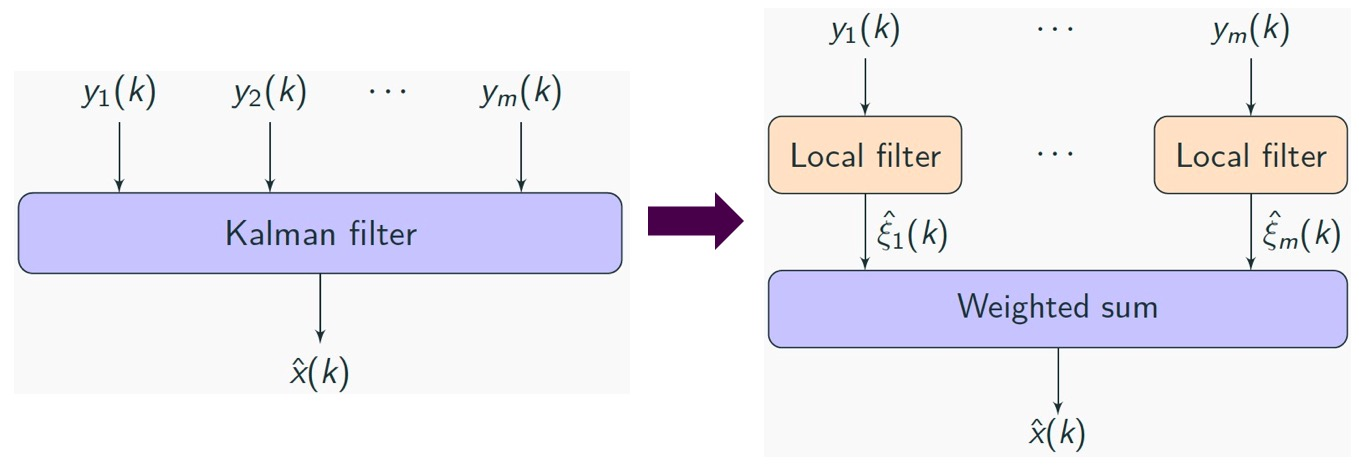
\includegraphics[width=1.0\textwidth]{pic/decomp}
	  \end{frame}

	  \begin{frame}{Decomposition of Kalman filter}
	    \begin{itemize}
	      \item $(A,C)$ is observable.
		\begin{itemize}
		  \item[a)] $A-KCA$ has {\color{thupurple} $n$ distinct} eigenvalues: $A-KCA=V\Lambda V^{-1}$;
		  \item[b)] $A-KCA$ and $A$ {\color{thupurple}do not share} any eigenvalues.
		\end{itemize}
	      \item {\textbf{[Mo2016]}}:
		The Kalman filter can be losslessly decomposed as a linear combination of local filters :
		\begin{align*}
		  \hat \xi_i(k+1)&=\Lambda\hat \xi_i(k)+\1_ny_i(k+1),\\
		  \hat x(k)&=\sum_{i=1}^m F_i\hat \xi_i(k),
		\end{align*}
		where $K=[K_1,\cdots,K_m]$, $F_i=V \diag(V^{-1}K_i)$, and {\color{thupurple}$\hat\xi_i(k)$ is a stable estimate of $G_ix(k)$}. 
	    \end{itemize}
	  \end{frame}

	  \begin{frame}{Decomposition of Kalman filter}
	    \begin{itemize}
	      \item Each sensor runs the following filter:
		\begin{align*}
		  \hat\xi_i(k+1)=\textcolor{thupurple}{\Lambda}\xi_i(k)+\1_n \textcolor{red}{y_i(k+1)},
		\end{align*}
		where $y_i(k+1)$ is not stable.
	      \item With an equivalent transformation $z_i(k)=y_i(k+1)-\beta^T\hat\xi_i(k)$, we have
		\begin{align*}
		  \hat\xi_i(k+1)&=\textcolor{red}{(\Lambda+\1_n\beta^T)}\hat\xi_i(k)+\1_n\textcolor{thupurple}{z_i(k)}\\
				&=\textcolor{red}{S}\hat\xi_i(k)+\1_n\textcolor{thupurple}{z_i(k)},
		\end{align*}
		where $\sum_{i=1}^n \beta_i(A-\lambda_i I)^{-1}=I$ and $S\triangleq \Lambda+\1_n\beta^T$.
	      \item {\color{thupurple}$z_i(k)$ is stable}, i.e. $cov(z_i(k))$ is bounded.
	      \item \textcolor{thupurple}{stable system matrix} + \textcolor{red}{unstable update} $\rightarrow$ \textcolor{red}{unstable system matrix} + \textcolor{thupurple}{stable update}.
	    \end{itemize}
	  \end{frame}

	  %\begin{frame}{Decomposition of Kalman filter}
	  %	\centering
	  %	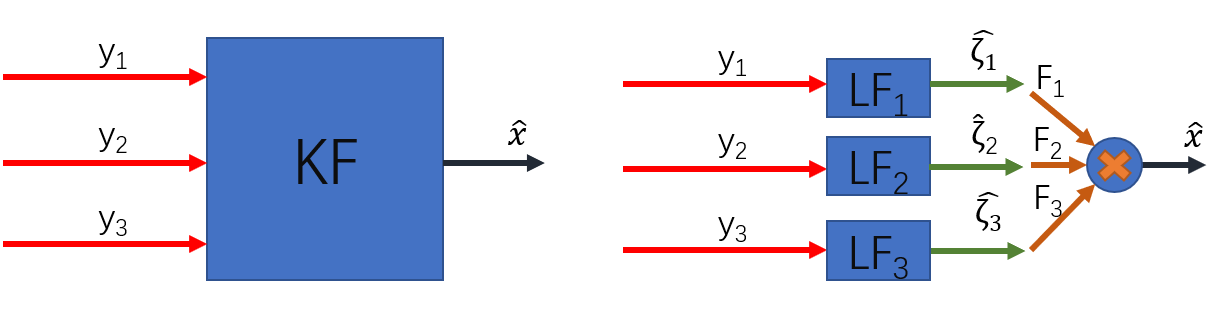
\includegraphics[width=0.75\textwidth]{pic/filter.png}
	  %	
	  %	\begin{itemize}
	  %		\item The Kalman filter can be \alert{losslessly} decomposed into a set of local filters \cite{Mo2016}:
	  %		\begin{align*}
	  %		\hat \xi_i(k+1)&=\Lambda\hat \xi_i(k)+\1_ny_i(k+1),\\
	  %		\hat x(k)&=\sum_{i=1}^m F_i\hat \xi_i(k).
	  %		\end{align*}
	  %	\end{itemize}
	  %\end{frame}

	  \begin{frame}{Decomposition of Kalman filter}
	    \begin{itemize}
	      \item Each sensor runs a local filter:
		\begin{align*}
		  \hat \xi_i(k+1)&=S\hat\xi_i(k)+\1_n z_i(k)
		\end{align*}

	      \item Decomposition of Kalman filter:
		\begin{align}
		  \begin{bmatrix}
		    \hat \xi_1(k+1) \\
		    \vdots\\
		    \hat \xi_m(k+1)
		  \end{bmatrix}&=
		  (I_m\otimes S)
		  \begin{bmatrix}
		    \hat \xi_1(k) \\
		    \vdots\\
		    \hat \xi_m(k)
		  \end{bmatrix}+
		  (I_m\otimes \1_n)
		  \begin{bmatrix}
		    z_1(k) \\
		    \vdots\\
		    z_m(k)
		  \end{bmatrix},\\
		  \hat{x}(k) &= F
		  \begin{bmatrix}
		    \hat \xi_1(k) \\
		    \vdots\\
		    \hat \xi_m(k)
		  \end{bmatrix}.
		\end{align}
	    \end{itemize}
	  \end{frame}

	  \begin{frame}{Distributed implementation of Kalman filter}
	    \begin{itemize}
	      \item Let sensor $i$ estimate $\frac{1}{m}\hat\xi_j(k)$, denoted by $\eta_{i,j}(k)$:
		\begin{equation*}
		  \begin{split}
		    \begin{bmatrix}
		      \eta_{i,1}(k+1) \\
		      \vdots\\
		      \eta_{i,m}(k+1)
		    \end{bmatrix}&=
		    (I_m\otimes S)
		    \begin{bmatrix}
		      \eta_{i,1}(k) \\
		      \vdots\\
		      \eta_{i,m}(k)
		    \end{bmatrix}+Bu_i(k)+
		    (e_i\otimes \1_n)z_i(k),\\
		    \breve{x_i}(k) &= mF
		    \begin{bmatrix}
		      \eta_{i,1}(k) \\
		      \vdots\\
		      \eta_{i,m}(k)
		    \end{bmatrix}.
		  \end{split}
		\end{equation*}
	      \item Matrix form:
		\begin{align*}
		  \eta_i(k+1) &=\tilde{S} \eta_i(k) + \tilde{B}u_i(k)+\textcolor{thupurple}{L_iz_i(k)}.
		\end{align*}
	    \end{itemize}
	  \end{frame}

	  \begin{frame}{Linear system synchronization}	
	    \begin{itemize}
	      \item Let us consider the synchronization of the following LTI system:
		\begin{align}\label{eqn:linear}
		  \eta_i(k+1) &= \tilde{S}\eta_i(k) + \tilde{B}u_i(k), \;\forall i\in\mathcal{V},
		\end{align}
	      \item \textit{Strong} synchronization:
		\begin{enumerate}
		  \item[1)]\textbf{Consistency:} the average of local states keeps consistent throughout the execution, i.e., 
		    \begin{equation}\label{eqn:consistency}
		      \textcolor{thupurple}{\sum_{i=1}^{m}\bar{\eta}(k+1) =\tilde{S}\sum_{i=1}^{m}\bar{\eta}(k).}
		    \end{equation}
		  \item[2)]\textbf{Exponential Stability:} agents exponentially reach consensus in the mean square sense, i.e., there exists $c>0$ and $\rho\in(0,1)$ such that 
		    \begin{equation}\label{eqn:consensus}
		      \textcolor{thupurple}{\mathbb{E}[||\eta_i(k)-\bar{\eta}(k)||^2] \leq c\rho^{k}, \;\forall i\in\mathcal{V}.}
		    \end{equation}
		\end{enumerate}
	    \end{itemize}
	  \end{frame}

	  \begin{frame}{Linear system synchronization}	
	    \begin{itemize}
	      \item {\textbf{[You2011]}}: Consider the control protocol:
		\begin{align*}
		  u_i(k)&=\sum_{j=1}^m a_{ij}(\Gamma \eta_j(k)-\Gamma \eta_i(k)).
		\end{align*}
	      \item In undirected graphs, the discrete-time multi-agent systems are consensusable with the protocol above if
		\begin{itemize}
		  \item $(S,B)$ is a controllable pair;
		  \item The product of the unstable eigenvalues of $S$ satisfies $$\prod_{j}|\lambda_j^u(S)|<\frac{1+\mu_2/\mu_m}{1-\mu_2/\mu_m},$$
		\end{itemize}
		where $0=\mu_1\leq \mu_2 \leq \cdots \leq \mu_m$ are the eigenvalues of $\mathcal{L}$.
	      \item We can find a common gain $\Gamma$ such that $\rho(S-\mu_j B \Gamma)<1$ for all $j=2,...,m.$
	    \end{itemize}
	  \end{frame}

	  %\section{Consensus}
	  %\begin{frame}{Consensus algorithm}
	  %	\begin{itemize}
	  %		\item 
	  %		\begin{align*}
	  %		x_i(k+1)&=Ax_i(k)+Bu_i(k),i=1,2,\cdots,m\\
	  %		u_i(k)&=\sum_{j=1}^m a_{ij}(\Gamma x_j(k)-\Gamma x_i(k)).
	  %		\end{align*}
	  %		\item In \alert{undirected} graphs \cite{You2011}, the discrete-time multi-agent systems are \alert{consensusable} with the protocol above \alert{if and only if}:
	  %		\begin{itemize}
	  %			\item $(A,B)$ is a controllable pair;
	  %			\item $\prod_{j}|\lambda_j^u(A)|<\frac{1+\mu_2/\mu_m}{1-\mu_2/\mu_m}$.
	  %		\end{itemize}
	  %	\end{itemize}
	  %\end{frame}
	  %
	  %\begin{frame}{Consensus algorithm}
	  %	\begin{columns}[c]
	  %		\column{6cm}
	  %		\begin{itemize}
	  %			\item \alert{Globally converge} to the average of all agents.
	  %			\item \alert{Low requirements on the topology} of the communication graph \cite{You2011}.
	  %			\item Show excellence in linear system \alert{synchronization}.
	  %		\end{itemize}
	  %		\column{6cm}
	  %		\begin{figure}
	  %			\centering
	  %			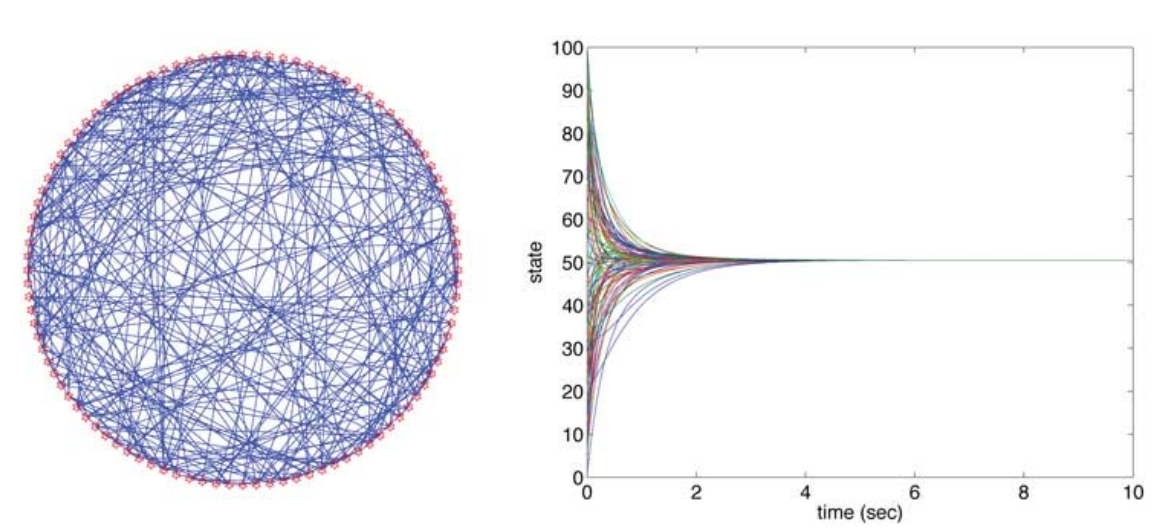
\includegraphics[width=1\textwidth]{pic/consensus_1.png}
	  %			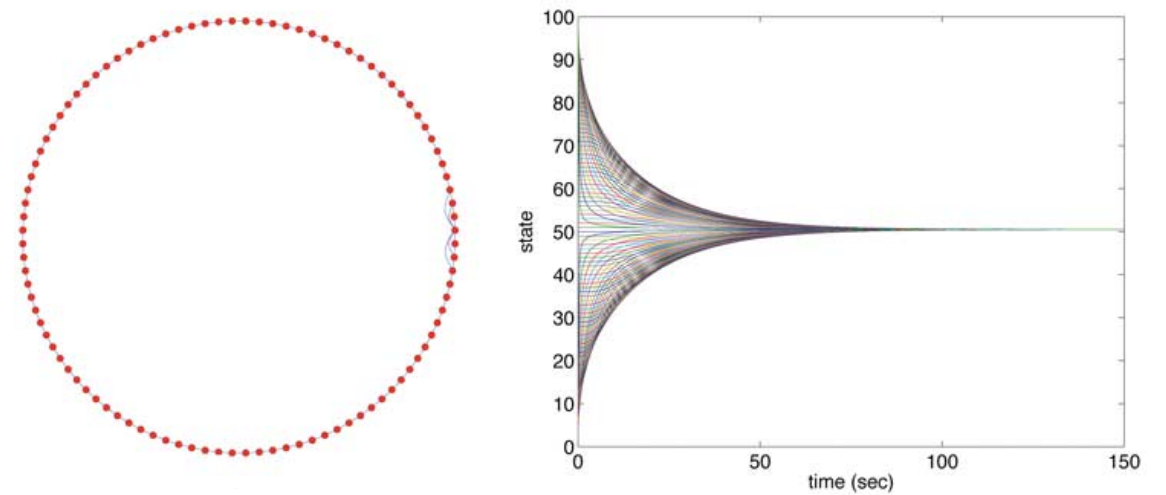
\includegraphics[width=1\textwidth]{pic/consensus_2.png}
	  %			\caption{Topology and state evolution \cite{Murray2007}}
	  %		\end{figure}
	  %	\end{columns}
	  %\end{frame}


	  \begin{frame}{Our algorithm}
	    Apply the linear system synchronization algorithm to solve the distributed estimation problem:
	    \begin{enumerate}
	      \item \textcolor{thupurple}{Update the residual} $z_i(k)$.
		\begin{align*}
		  z_i(k)&=y_i(k+1)-\beta^T\hat\xi_i(k),\\
		  \hat\xi_i(k+1)&=S\hat\xi_i(k)+\1_nz_i(k).
		\end{align*}
	      \item Run the \textcolor{thupurple}{sychronization} algorithm.
		\begin{align*}
		  \eta_i(k+1)&=(I_m\otimes S)\eta_i(k) +(e_i\otimes\1_n)z_i(k)+
		  B\sum_{i=1}^m a_{ij}(\Gamma \eta_j(k)-\Gamma \eta_i(k)).
		\end{align*}
	      \item Update the state estimation:
		\begin{align*}
		  \breve x_i(k+1)=mF\eta_i(k+1).
		\end{align*}
	      \item Transmit a new message $\Delta_i(k+1)$ to neighbors.
	    \end{enumerate}
	  \end{frame}

	  \begin{frame}{Our algorithm}
	    \begin{figure}
	      \centering
	      \resizebox{0.63\textwidth}{!}{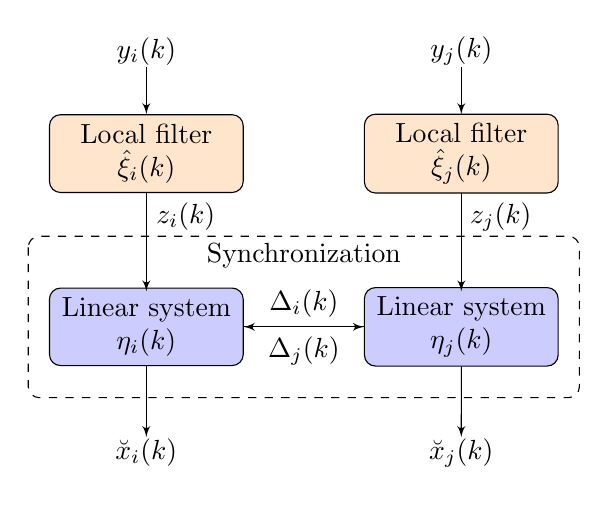
\begin{tikzpicture}[auto, node distance=1.8cm,>=latex']

\node at (0,3.5) {$y_i(k)$};
\node at (4,3.5) {$y_j(k)$};

\draw [->] (0,3.3) -- (0,2.7);
\draw [->] (4,3.3) -- (4,2.7);

\node [sensor,align=center] (est1) {Linear system\\$\eta_{i}(k)$};
\node [sensor, right of=est1,node distance=4cm,align=center] (est2) {Linear system\\$\eta_{j}(k)$};
\node [est,above of=est1,align=center,node distance=2.2cm] (sensor1) {Local filter\\$\hat{\xi}_i(k)$};
\node [est,above of=est2,align=center,node distance=2.2cm] (sensor2) {Local filter\\$\hat{\xi}_j(k)$};


\draw [->] (0,1.7) --  (0,0.45);
\draw [->] (4,1.7) -- (4,0.45);
%\\$y_i(k)$\\\quad\\\quad\\$\hat{\xi}_i(k)$

\node at (0.5,1.4) {$z_i(k)$};
\node at (4.5,1.4) {$z_j(k)$};

\draw [->] (est1) -- node {$\Delta_i(k)$} (est2);
\draw [->] (est2) -- node {$\Delta_j(k)$} (est1);

\draw [dashed,rounded corners](-1.5,1.15) rectangle (5.5,-0.9);

\node at (2,0.9) {Synchronization};

\draw [->] (est1) --  (0,-1.4);
\draw [->] (est2) -- (4,-1.4);


\node at (0,-1.6) {$\breve{x}_i(k)$};
\node at (4,-1.6) {$\breve{x}_j(k)$};
\end{tikzpicture}
}
	      %\caption{The information flow of centralized Kalman filter.}
	    \end{figure}
	  \end{frame}

	  \begin{frame}{Our algorithm}
	    \begin{itemize}
	      \item The proposed algorithm yields a \textcolor{thupurple}{stable estimator} at each sensor side:
		\begin{enumerate}
		  \item[1)] the average of local estimates from all sensor coincides with the optimal Kalman estimate, namely
		    \begin{equation}
		      \frac{1}{m}\sum_{i=1}^m \breve{x}_i(k)=\hat{x}(k);
		    \end{equation}
		  \item[2)] the error covariance of each local estimate is bounded. Moreover, the asymptotic error covariance can be exactly derived.
		\end{enumerate} 
	    \end{itemize}
	  \end{frame}

	  \begin{frame}{Recall linear system synchronization}
	    \begin{itemize}
	      \item Bridge the fields of distributed estimation and linear system synchronization.
	    \end{itemize}
	    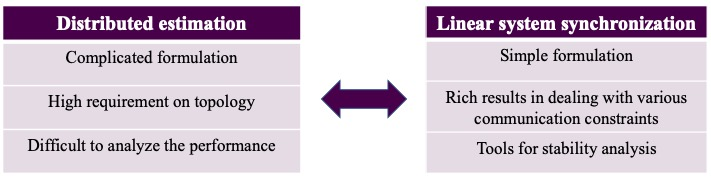
\includegraphics[width=1\textwidth]{pic/bridge}
	    \begin{itemize}
	      \item Markovian switching topology [You2013]; Random link failures [Xu2019]...
	    \end{itemize}
	  \end{frame}

	  \begin{frame}{Numerical example}
	    \begin{columns}[c]
	      \column{5cm}
	      \begin{align*}
		A&=\begin{bmatrix}
		  0.9 & 0\\
		  0 & 1.1
		\end{bmatrix},\\
		  C&=\begin{bmatrix}
		    1 & 0\\
		    0 & 1\\
		    1 & 1\\
		    1 & -1
		  \end{bmatrix},\\
		    Q&=0.25I_2, R=4I_4.
		  \end{align*}
		  \column{7cm}
		  \begin{figure}
		    \centering
		    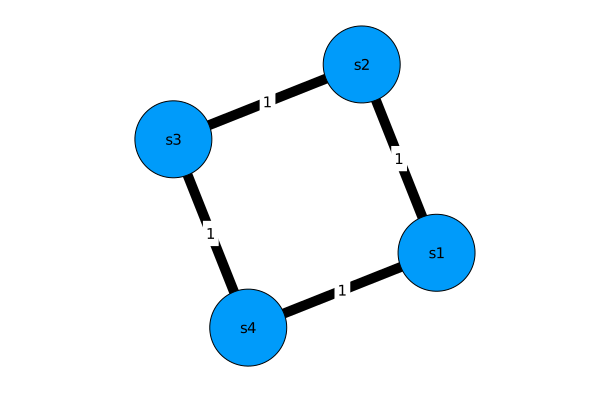
\includegraphics[width=1\textwidth]{pic/topology.png}
		    \caption{Topology of the communication graph.}
		  \end{figure}
		\end{columns}
	      \end{frame}

	      \begin{frame}{Simulation result}
		\begin{figure}
		  \centering
		  \scalebox{0.7}{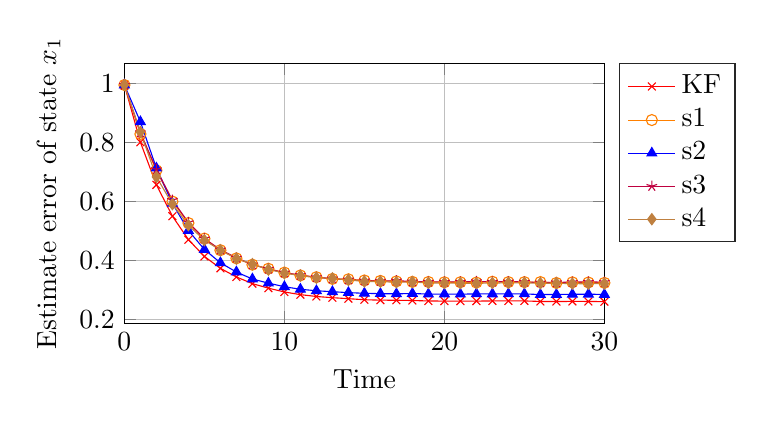
\begin{tikzpicture}
\begin{axis}[%
width=2.4in,
height=1.3in,
scale only axis,
xmin=0,
xmax=30,
xlabel={Time},
ylabel={Estimate error of state $x_1$},
axis background/.style={fill=white},
xmajorgrids,
ymajorgrids,
legend style={legend cell align=left, align=left, draw=white!15!black},
legend pos={outer north east}
]
    \addplot[color={red}, mark={x}]
        coordinates {
            (0,0.9938736998561463)
            (1,0.7998312599375371)
            (2,0.6552675534350793)
            (3,0.5491314278478721)
            (4,0.4694799147910701)
            (5,0.4124624385056815)
            (6,0.3721888244880748)
            (7,0.342896253109788)
            (8,0.32026764135190405)
            (9,0.304892836991136)
            (10,0.29200384686246134)
            (11,0.28297379643031495)
            (12,0.27668961019129906)
            (13,0.2725977233559627)
            (14,0.26926981656843674)
            (15,0.26564889420782367)
            (16,0.2642539514894093)
            (17,0.2639247767173576)
            (18,0.26304078533210873)
            (19,0.26151391429325116)
            (20,0.2610055846609784)
            (21,0.2610801563062564)
            (22,0.26100407922942226)
            (23,0.26165224459393305)
            (24,0.26175778384304416)
            (25,0.26161200966182985)
            (26,0.2598879117677957)
            (27,0.2595078795770665)
            (28,0.26005225008966654)
            (29,0.2598112548773231)
            (30,0.2592574531270815)
            (31,0.2602334111819597)
            (32,0.2608806386097496)
            (33,0.26174960735116337)
            (34,0.26113366656759207)
            (35,0.2599380111371554)
            (36,0.25901760236121385)
            (37,0.25846447356766505)
            (38,0.25883301142410664)
            (39,0.25967947640742967)
            (40,0.25970890124636914)
            (41,0.26073512429871326)
            (42,0.2601919812570974)
            (43,0.2595060207502124)
            (44,0.2599877309012237)
            (45,0.26116255846121617)
            (46,0.2601682050494274)
            (47,0.26074856825442194)
            (48,0.26054896536446837)
            (49,0.2601874302567705)
            (50,0.25943557666834594)
        }
        ;
    \addlegendentry {KF}
    \addplot[color={orange}, mark={o}]
        coordinates {
            (0,0.9938736998561463)
            (1,0.8276013460811993)
            (2,0.7043486327056803)
            (3,0.598584203091598)
            (4,0.5256456013961409)
            (5,0.4730480973677678)
            (6,0.4336170518531029)
            (7,0.4059034949821229)
            (8,0.38459840869216727)
            (9,0.3707972358283984)
            (10,0.3576809276665771)
            (11,0.3481287936793677)
            (12,0.34212296014945826)
            (13,0.3364236636364027)
            (14,0.3350756942959627)
            (15,0.3311186634236469)
            (16,0.32952873899516033)
            (17,0.32796544243410486)
            (18,0.32636001167475454)
            (19,0.3259008402733645)
            (20,0.324931831968992)
            (21,0.32505003087796047)
            (22,0.3240023762232875)
            (23,0.32674547129850556)
            (24,0.32549833224117186)
            (25,0.32541337948482446)
            (26,0.3256170939348204)
            (27,0.32258826225614884)
            (28,0.32475442151198264)
            (29,0.32418172225095204)
            (30,0.3228438634630245)
            (31,0.3245833904161518)
            (32,0.32500396513177804)
            (33,0.3259541718782387)
            (34,0.3254925957091615)
            (35,0.3236953376446919)
            (36,0.32166280136415326)
            (37,0.3239702698216697)
            (38,0.3219689757670435)
            (39,0.323387896278814)
            (40,0.32391586660665317)
            (41,0.3240977569129136)
            (42,0.3260637745636904)
            (43,0.32503775663745)
            (44,0.32551120806489114)
            (45,0.325346440605765)
            (46,0.3248096756157781)
            (47,0.32487774492925325)
            (48,0.3261323039272188)
            (49,0.3235797365529704)
            (50,0.32321206752387277)
        }
        ;
    \addlegendentry {s1}
    \addplot[color={blue}, mark={triangle*}]
        coordinates {
            (0,0.9938736998561463)
            (1,0.8690457045552045)
            (2,0.7119279890009231)
            (3,0.5923819128150415)
            (4,0.5002457913220736)
            (5,0.4361920096215039)
            (6,0.3908883806261038)
            (7,0.35971173152747266)
            (8,0.33586387346463686)
            (9,0.32193945687672326)
            (10,0.3098135515134442)
            (11,0.3011339823202175)
            (12,0.29610710981458166)
            (13,0.29285945258554247)
            (14,0.2897779144208205)
            (15,0.2874991925430223)
            (16,0.28628039600952054)
            (17,0.28568821532927563)
            (18,0.28685086136950994)
            (19,0.28485839609925)
            (20,0.2849303514904291)
            (21,0.28451418544906204)
            (22,0.28550706513452473)
            (23,0.2853174069695211)
            (24,0.2856483722520482)
            (25,0.28536050754699527)
            (26,0.28328233983362844)
            (27,0.2833966472055331)
            (28,0.284043001830299)
            (29,0.28450493552375616)
            (30,0.283564619218778)
            (31,0.28495500414053226)
            (32,0.28530582895421325)
            (33,0.2865198555419734)
            (34,0.285989322134304)
            (35,0.2849749072429814)
            (36,0.28428603282279347)
            (37,0.2822839434538884)
            (38,0.2830552528856996)
            (39,0.28330785066683134)
            (40,0.283483264659842)
            (41,0.2856890215000939)
            (42,0.28421182254422833)
            (43,0.28357028822809305)
            (44,0.28369368444314297)
            (45,0.2850311736621484)
            (46,0.2842881201560302)
            (47,0.28521695596164054)
            (48,0.2847614590394634)
            (49,0.2850139510069791)
            (50,0.28485430954222263)
        }
        ;
    \addlegendentry {s2}
    \addplot[color={purple}, mark={star}]
        coordinates {
            (0,0.9938736998561463)
            (1,0.8325859476122843)
            (2,0.7073897136050656)
            (3,0.6034749935033639)
            (4,0.5275726228149147)
            (5,0.4725831082570765)
            (6,0.43547543835225033)
            (7,0.4078811305071094)
            (8,0.384705576325829)
            (9,0.370092672145898)
            (10,0.3572377352896849)
            (11,0.349201326989582)
            (12,0.3417428545235937)
            (13,0.3373026560410906)
            (14,0.33371971405717166)
            (15,0.33072298139747197)
            (16,0.32873189771116545)
            (17,0.33046645481974085)
            (18,0.32733914555930327)
            (19,0.326086471481113)
            (20,0.32611934637142864)
            (21,0.3264161245451283)
            (22,0.32789165317837493)
            (23,0.32611000923119565)
            (24,0.3270265982465661)
            (25,0.326090148190561)
            (26,0.32373559803173)
            (27,0.3242916189064993)
            (28,0.32542452673580397)
            (29,0.3260128343215159)
            (30,0.3253239754809772)
            (31,0.32603116954327516)
            (32,0.3256400510268415)
            (33,0.3282706785555161)
            (34,0.3260292021373245)
            (35,0.32576855983196407)
            (36,0.3249511540567645)
            (37,0.3230299296021767)
            (38,0.32419268373687665)
            (39,0.32512358156992793)
            (40,0.32661239445773804)
            (41,0.3266854217002811)
            (42,0.3238935627542437)
            (43,0.3229594890948283)
            (44,0.32418033596696927)
            (45,0.32520744181469524)
            (46,0.3249416786945417)
            (47,0.3257839102748252)
            (48,0.32563852090666146)
            (49,0.32690816878238493)
            (50,0.32577337757982483)
        }
        ;
    \addlegendentry {s3}
    \addplot[color={brown}, mark={diamond*}]
        coordinates {
            (0,0.9938736998561463)
            (1,0.8343473999900486)
            (2,0.6822833021672857)
            (3,0.5899142707956274)
            (4,0.5182987446558422)
            (5,0.4675908730658054)
            (6,0.43350277481559124)
            (7,0.40547354140469666)
            (8,0.3862570601591901)
            (9,0.36807970671848506)
            (10,0.3561553044134684)
            (11,0.3471982591140287)
            (12,0.34027389213798453)
            (13,0.3379929251594904)
            (14,0.33278011147647396)
            (15,0.327625385530501)
            (16,0.3270821358208276)
            (17,0.32497323000304207)
            (18,0.32555662692690907)
            (19,0.32276996028079447)
            (20,0.32215457434325434)
            (21,0.3217828459857988)
            (22,0.3213620072692803)
            (23,0.32229698073255747)
            (24,0.3229285159012965)
            (25,0.32293444859886605)
            (26,0.3214561133226882)
            (27,0.3216030504550832)
            (28,0.32021398223117714)
            (29,0.31985569158716703)
            (30,0.3205502791012525)
            (31,0.32073406012314265)
            (32,0.3219379552948372)
            (33,0.32103738203264903)
            (34,0.32159115134826693)
            (35,0.31934458799994936)
            (36,0.3205593093017057)
            (37,0.31870880349791386)
            (38,0.32081053658788317)
            (39,0.3218149433555171)
            (40,0.3197246279159553)
            (41,0.3211652693961577)
            (42,0.32126305883557493)
            (43,0.3211102597500812)
            (44,0.3204900260033881)
            (45,0.323094674930004)
            (46,0.32125045787242584)
            (47,0.3212528756591601)
            (48,0.32056885659423623)
            (49,0.320213202267437)
            (50,0.31999954839432815)
        }
        ;
    \addlegendentry {s4}
\end{axis}
\end{tikzpicture}
}
		  \scalebox{0.7}{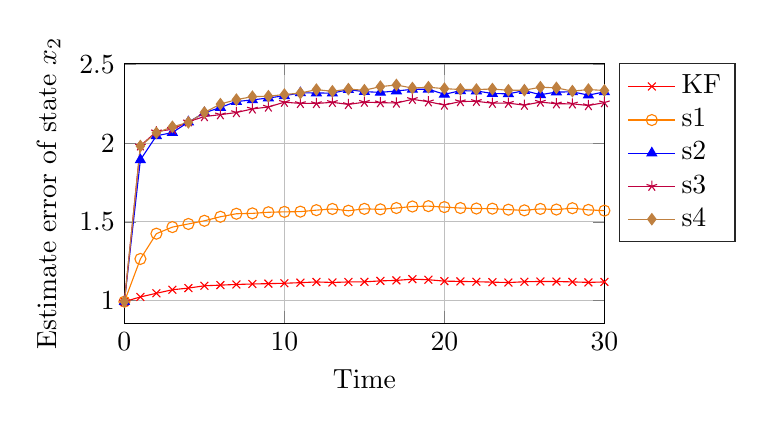
\begin{tikzpicture}
\begin{axis}[%
width=2.4in,
height=1.3in,
scale only axis,
xmin=0,
xmax=30,
xlabel={Time},
ylabel={Estimate error of state $x_2$},
axis background/.style={fill=white},
xmajorgrids,
ymajorgrids,
legend style={legend cell align=left, align=left, draw=white!15!black},
legend pos={outer north east}
]
    \addplot[color={red}, mark={x}]
        coordinates {
            (0,0.9943765995349962)
            (1,1.0241254689704056)
            (2,1.0473887499847159)
            (3,1.0697339448807577)
            (4,1.0803713746007921)
            (5,1.0949033915033333)
            (6,1.0991482380149056)
            (7,1.1034194862558937)
            (8,1.106307793947288)
            (9,1.1085925380380288)
            (10,1.110999599114129)
            (11,1.1147645806759343)
            (12,1.1193703731575648)
            (13,1.116094933319016)
            (14,1.1192249437084907)
            (15,1.1199115573191498)
            (16,1.1260096469155687)
            (17,1.1291450572405135)
            (18,1.136950337574846)
            (19,1.133455361109355)
            (20,1.1244685761514959)
            (21,1.1227919434732434)
            (22,1.1206090843375092)
            (23,1.1180481048662483)
            (24,1.1155404791626586)
            (25,1.1204428581200438)
            (26,1.1224462151114232)
            (27,1.121752685683367)
            (28,1.1196943320049257)
            (29,1.1164613963806695)
            (30,1.1193740859610601)
            (31,1.1196678829620261)
            (32,1.1262821415531057)
            (33,1.1156317612924114)
            (34,1.116567512625055)
            (35,1.116742559368047)
            (36,1.117315577996865)
            (37,1.118028323124454)
            (38,1.1164678892437345)
            (39,1.117983506365516)
            (40,1.123098865189546)
            (41,1.1230946876927135)
            (42,1.1225522521222113)
            (43,1.1224618836995262)
            (44,1.1238984888915637)
            (45,1.125901217233803)
            (46,1.1226315332791659)
            (47,1.119965687831627)
            (48,1.1193711594564655)
            (49,1.1226049410413392)
            (50,1.1241068397421996)
        }
        ;
    \addlegendentry {KF}
    \addplot[color={orange}, mark={o}]
        coordinates {
            (0,0.9943765995349962)
            (1,1.2652924039335356)
            (2,1.4256320040837056)
            (3,1.4673510411562172)
            (4,1.4873395687011577)
            (5,1.5073301774920105)
            (6,1.5329161641112685)
            (7,1.5520030589757723)
            (8,1.554391863843294)
            (9,1.5615200183722036)
            (10,1.563923717117754)
            (11,1.5653870801152323)
            (12,1.574879924241972)
            (13,1.5825303535941295)
            (14,1.5711163184525245)
            (15,1.5831105788545525)
            (16,1.5799868657614462)
            (17,1.5882189783567848)
            (18,1.5979613761646876)
            (19,1.6003075631065073)
            (20,1.5941329592447682)
            (21,1.588284581504355)
            (22,1.5851274627279721)
            (23,1.584373968832322)
            (24,1.577858666299255)
            (25,1.5735674219348068)
            (26,1.5827615472696204)
            (27,1.5786961819804337)
            (28,1.587122886228931)
            (29,1.5765449008480295)
            (30,1.571758603170185)
            (31,1.5722071728043354)
            (32,1.5790341798123353)
            (33,1.5937749764613511)
            (34,1.5745873058034463)
            (35,1.5701470146906793)
            (36,1.5669255079112894)
            (37,1.5699117333623531)
            (38,1.57213903822218)
            (39,1.5750483423635424)
            (40,1.5761992587434166)
            (41,1.5812174368332743)
            (42,1.5817244605547665)
            (43,1.586364793112144)
            (44,1.5853213582576369)
            (45,1.5866770960927927)
            (46,1.5821300768923279)
            (47,1.5851061919445362)
            (48,1.5826051452764909)
            (49,1.572164251666703)
            (50,1.5822951282611506)
        }
        ;
    \addlegendentry {s1}
    \addplot[color={blue}, mark={triangle*}]
        coordinates {
            (0,0.9943765995349962)
            (1,1.8936625444249422)
            (2,2.0465205257360233)
            (3,2.066951276012711)
            (4,2.1338615693851746)
            (5,2.1922909740541803)
            (6,2.226487115248709)
            (7,2.263933580097268)
            (8,2.2742324432017647)
            (9,2.2866612655231235)
            (10,2.300561709236413)
            (11,2.3187874391349936)
            (12,2.3183107436885133)
            (13,2.3172153186124294)
            (14,2.339358433536219)
            (15,2.326601894094998)
            (16,2.322100645625816)
            (17,2.3311028833616803)
            (18,2.3412621523512342)
            (19,2.342196254698138)
            (20,2.309811332436182)
            (21,2.3326324701167347)
            (22,2.331147100728079)
            (23,2.314863629664187)
            (24,2.31285475802809)
            (25,2.3332171428385466)
            (26,2.3071309244263793)
            (27,2.3241146984247614)
            (28,2.3254061798842365)
            (29,2.304722589550026)
            (30,2.3250475757893168)
            (31,2.326875039249452)
            (32,2.347786042018165)
            (33,2.3050612298653994)
            (34,2.3143523106351727)
            (35,2.323050036506524)
            (36,2.3268902505681694)
            (37,2.326027817270796)
            (38,2.3264477462757323)
            (39,2.3118714464205596)
            (40,2.329829962182898)
            (41,2.313641678866345)
            (42,2.334185411755957)
            (43,2.3313963439610914)
            (44,2.319456118549934)
            (45,2.3358929879940047)
            (46,2.3168383584104326)
            (47,2.321115857214799)
            (48,2.3270072795412897)
            (49,2.3384601141712515)
            (50,2.318873680806025)
        }
        ;
    \addlegendentry {s2}
    \addplot[color={purple}, mark={star}]
        coordinates {
            (0,0.9943765995349962)
            (1,1.9828858762138304)
            (2,2.072953590569488)
            (3,2.0880223184728335)
            (4,2.1360134385063105)
            (5,2.168877836105569)
            (6,2.180518305551039)
            (7,2.194470270203278)
            (8,2.2170095545654873)
            (9,2.2294796048964476)
            (10,2.259813698050696)
            (11,2.252040729684584)
            (12,2.2518134092075446)
            (13,2.258969773117035)
            (14,2.2456372378476983)
            (15,2.260074704840985)
            (16,2.25690801887656)
            (17,2.2546645079335232)
            (18,2.2780084217125545)
            (19,2.2627407160130613)
            (20,2.241840788498835)
            (21,2.2639896937363018)
            (22,2.2653910716270422)
            (23,2.253397842090359)
            (24,2.253664694284399)
            (25,2.2409423831703603)
            (26,2.260721382240181)
            (27,2.2498742978256083)
            (28,2.249337306194815)
            (29,2.2387064936893575)
            (30,2.2572354436442903)
            (31,2.2559199593761075)
            (32,2.2629454575339145)
            (33,2.237792912635502)
            (34,2.259809633090449)
            (35,2.2600701221241586)
            (36,2.2590233377061026)
            (37,2.2566562394095957)
            (38,2.259200706317603)
            (39,2.2522596098668717)
            (40,2.271687711433266)
            (41,2.251367671607407)
            (42,2.2467096704728404)
            (43,2.2653285924423328)
            (44,2.249874385082106)
            (45,2.2693838984464265)
            (46,2.2443897174131746)
            (47,2.2700278666501776)
            (48,2.2596714046786364)
            (49,2.2710007617069685)
            (50,2.2585889284508913)
        }
        ;
    \addlegendentry {s3}
    \addplot[color={brown}, mark={diamond*}]
        coordinates {
            (0,0.9943765995349962)
            (1,1.9816540696459648)
            (2,2.0654615474192903)
            (3,2.1035165609535103)
            (4,2.1315441874490997)
            (5,2.194405042764902)
            (6,2.2477131762354583)
            (7,2.2761788789650046)
            (8,2.2947881679581665)
            (9,2.2977677725464183)
            (10,2.308375957467222)
            (11,2.317980480162738)
            (12,2.339427607324274)
            (13,2.32883551380075)
            (14,2.3427375592794983)
            (15,2.3356439111894307)
            (16,2.3585557228897294)
            (17,2.3690788525616533)
            (18,2.3493756113388495)
            (19,2.354762160569893)
            (20,2.3456192480187106)
            (21,2.3403966321669003)
            (22,2.340282752809893)
            (23,2.3432582094375234)
            (24,2.3354632251712575)
            (25,2.3358984300908086)
            (26,2.3548376694214577)
            (27,2.350751598558515)
            (28,2.330001313064622)
            (29,2.339936620551301)
            (30,2.334139579826345)
            (31,2.3296671247918894)
            (32,2.3477739816701084)
            (33,2.3372527594188757)
            (34,2.3294471328167496)
            (35,2.331507818950099)
            (36,2.3364833657462096)
            (37,2.3324300667271194)
            (38,2.3362024692199643)
            (39,2.3484213589008274)
            (40,2.332847142957334)
            (41,2.3589948008145787)
            (42,2.345722793829973)
            (43,2.3270312885418902)
            (44,2.3439433888447985)
            (45,2.3273308186147994)
            (46,2.36039655167833)
            (47,2.339409769673635)
            (48,2.336415886140528)
            (49,2.3442896822054715)
            (50,2.328126528073856)
        }
        ;
    \addlegendentry {s4}
\end{axis}
\end{tikzpicture}
}
		  \caption{Average mean square estimation error of state estimates under Kalman filter and local estimators in 10000 experiments.}
		\end{figure}
	      \end{frame}

	      \begin{frame}{Numerical example}
		We simulate the heat transfer process in a planar closed region:
		\begin{align*}
		  \frac{\partial u}{\partial t}=\alpha\Big(\frac{\partial^2u}{\partial x_1^2}+\frac{\partial^2u}{\partial x_2^2}\Big),
		\end{align*}
		with boundary conditions
		\begin{align*}
		  \frac{\partial u}{\partial x_1}\Big|_{t,0,x_2}=\frac{\partial u}{\partial x_1}\Big|_{t,l,x_2}=\frac{\partial u}{\partial x_2}\Big|_{t,x_1,0}=\frac{\partial u}{\partial x_2}\Big|_{t,x_1,l}=0,
		\end{align*}
	      \end{frame}

	      \begin{frame}{Simulation result}
		\begin{figure}[]
		  \centering
		  \includegraphics[width=0.6\textwidth]{pic/variance.pdf}
		  \caption{(a) Position and topology of $m$ sensors; (b) Centralized KF; (c) Local KF; (d) Our estimators in 10000 experiments.}
		  \label{fig:heatmap}
		\end{figure}
	      \end{frame}

	      \begin{frame}{Equipments}
		\begin{columns}[c]
		  \column{6cm}
		  \begin{itemize}
		    \item Hardware: 30 raspberry pis, power banks and sensors.
		    \item Software: batman-adv.
		      \begin{itemize}
			\item Operates entirely on layer 2.
			\item Supports 1000 nodes and beyond.
		      \end{itemize}
		    \item Goal: build a mesh network and perform various distributed tasks.
		  \end{itemize}
		  \column{6cm}
		  \begin{figure}
		    \centering
		    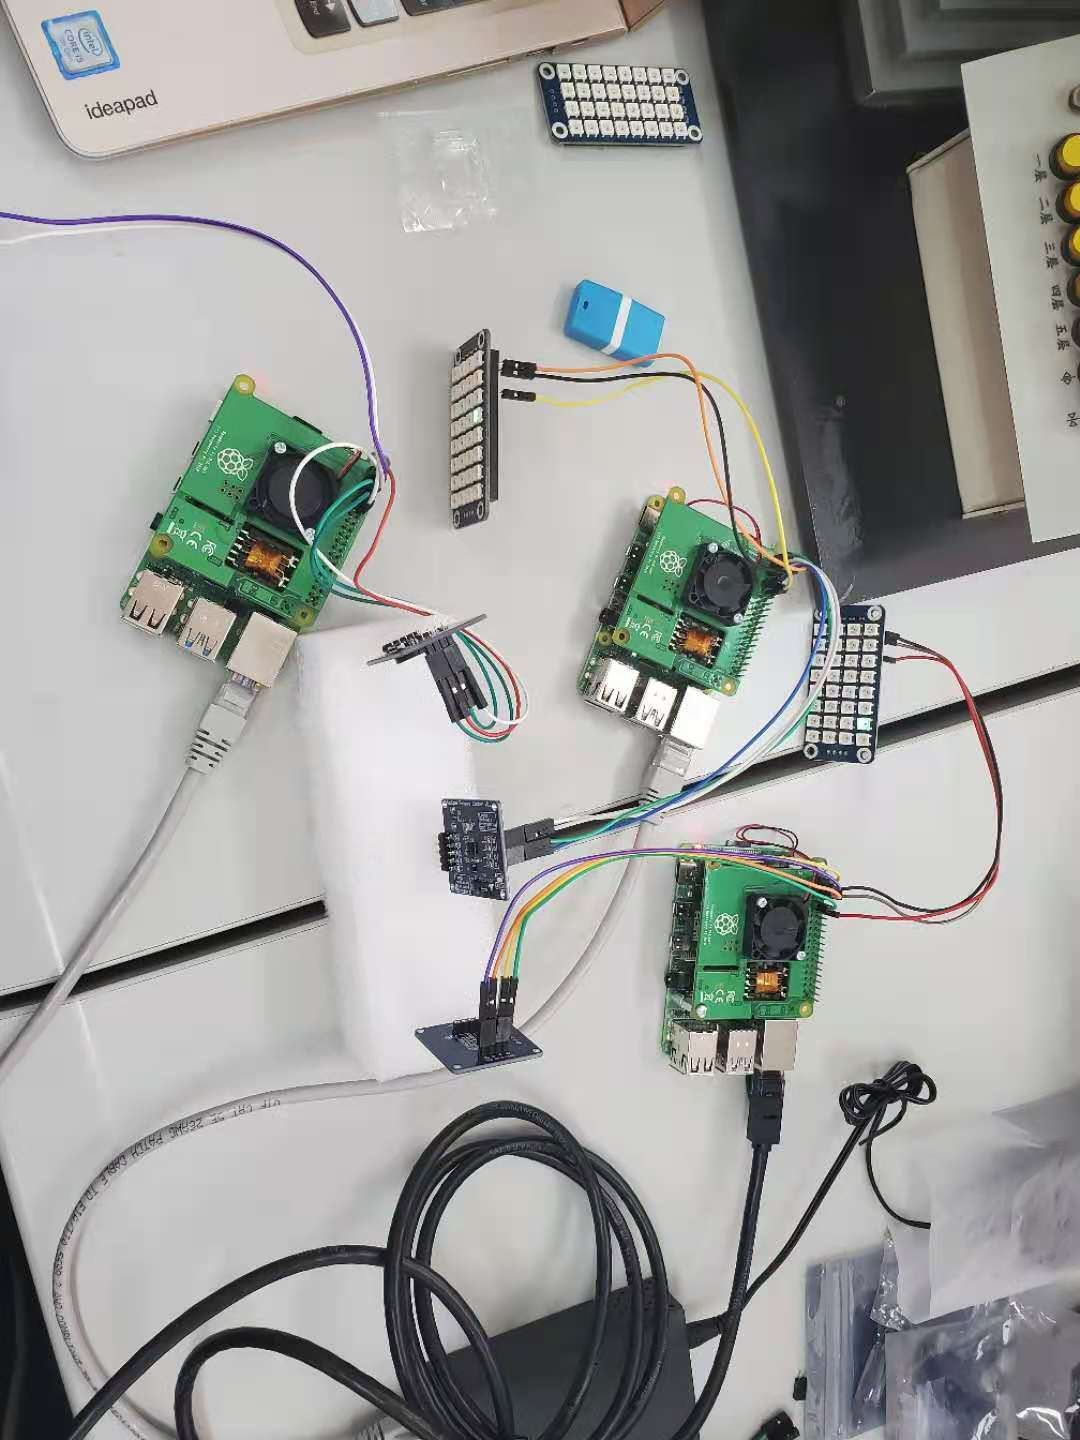
\includegraphics[width=0.6\textwidth,angle=90]{pic/rapberry_pi.jpg}
		    \caption{Available equipments.}
		  \end{figure}
		\end{columns}
	      \end{frame}

	      \begin{frame}{Batman-adv}
		\begin{figure}
		  \centering
		  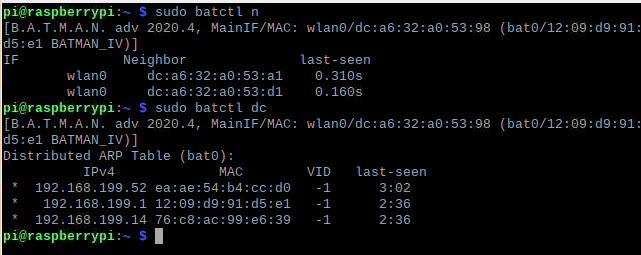
\includegraphics[width=0.7\textwidth]{pic/batman-adv.png}
		  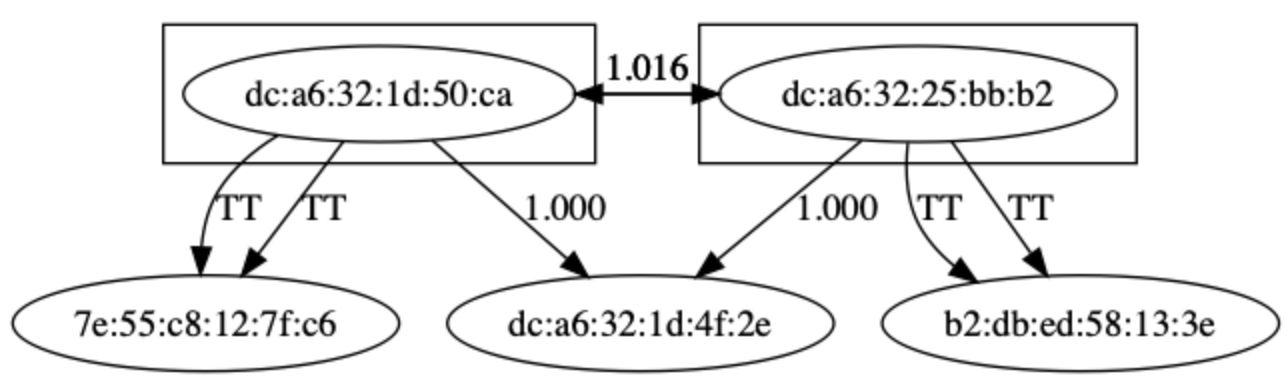
\includegraphics[width=0.5\textwidth]{pic/batman-topology.png}
		  \caption{Build mesh networks with batman-adv.}
		\end{figure}
		Future work:
		\begin{itemize}
		  \item Find ways to determine the topology.
		  \item Time synchronization.
		  \item Create a tool to visualize and monitor.
		\end{itemize}
	      \end{frame}

	      \begin{frame}{Reference}
		\footnotesize [1] Y. Mo, and E. Garone. ``Secure dynamic state estimation via local estimators." 2016 IEEE 55th Conference on Decision and Control (CDC). IEEE, 2016.

		[2] K. You, and L. Xie. ``Network topology and communication data rate for consensusability of discrete-time multi-agent systems." IEEE Transactions on Automatic Control 56.10 (2011): 2262-2275.

		[3] K. You, Z. Li, and L. Xie. ``Consensus condition for linear multi-agent systems over randomly switching topologies." Automatica 49.10 (2013): 3125-3132.

		[4] L. Xu, Y. Mo, and L. Xie. ``Distributed consensus over markovian packet loss channels." IEEE Transactions on Automatic Control 65.1 (2019): 279-286.
	      \end{frame}

	      \begin{frame}{Reference}
		J. Yan, X. Yang, Y. Mo, and K. You. ``A distributed implementation of steady-state Kalman filter." 

		\vspace{10pt}
		\centering
		
\includegraphics[width=0.3\textwidth]{pic/qr.jpeg}
	      \end{frame}


	      \begin{frame}{Experiment with Raspberry Pis}
		\begin{columns}[c]
		  \column{7cm}
		  \begin{itemize}
		    \item A mesh network is created over WiFi with batman-adv \cite{batman-adv}.
		    \item Batman-adv is an implementation of the Batman wireless routing protocol, which enables each Raspberry Pi to find and communicate with its neighbors.
		  \end{itemize}
		  \column{5cm}
		  \begin{figure}
		    \centering
		    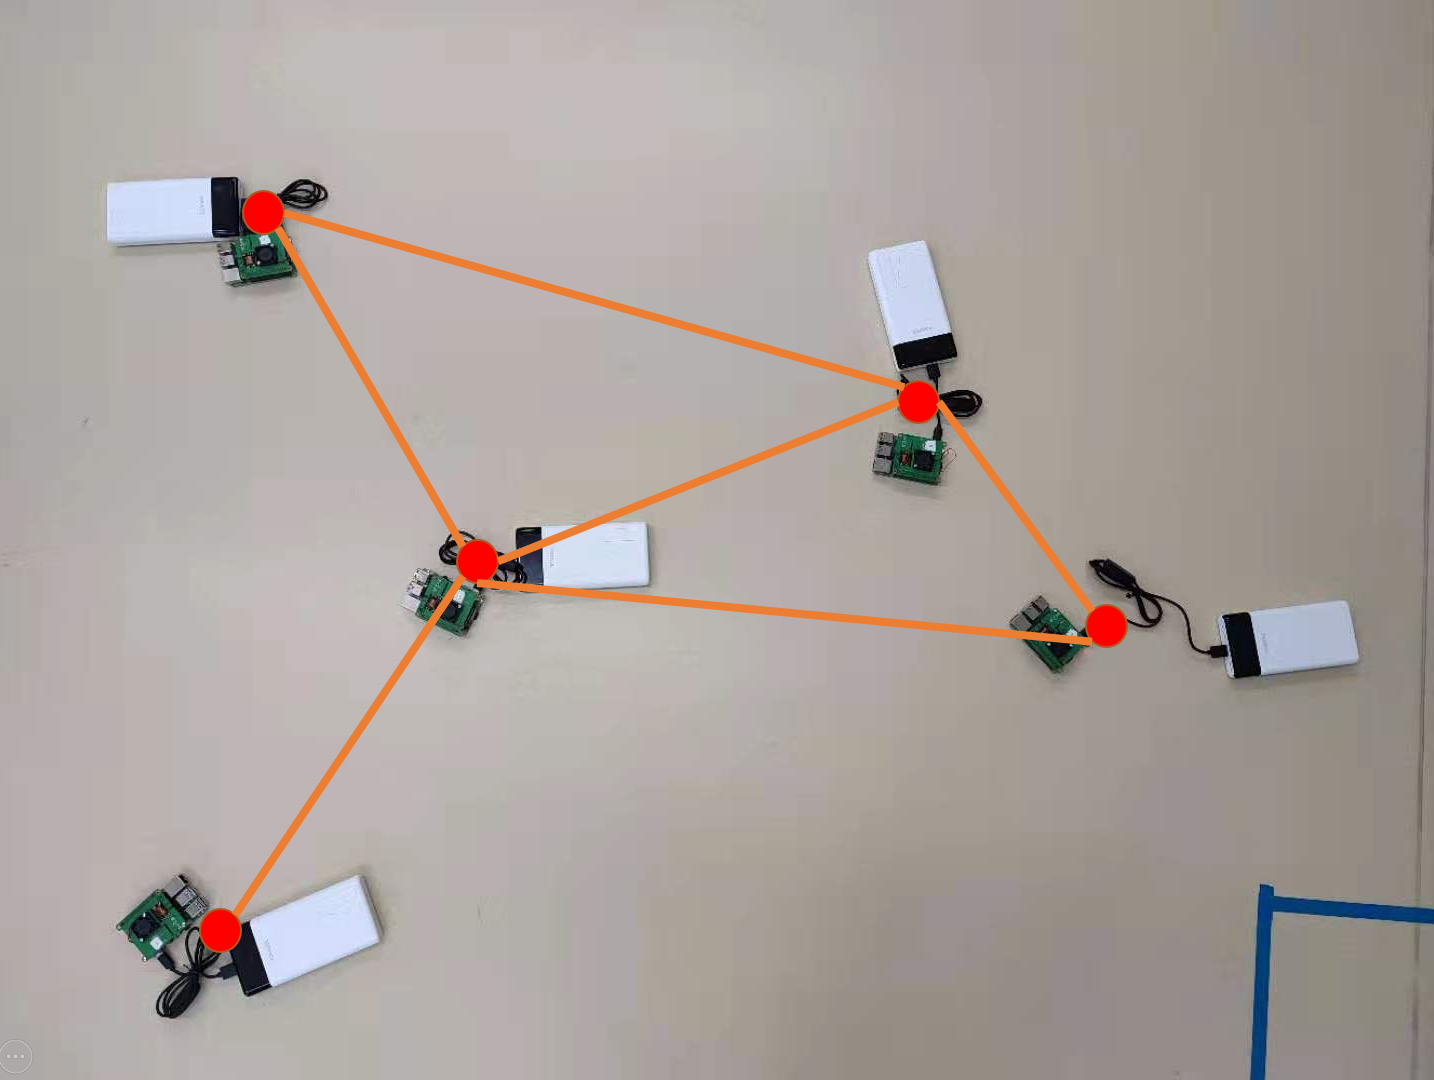
\includegraphics[width=1\textwidth]{pic/rpi_expriment.png}
		  \end{figure}
		\end{columns}
	      \end{frame}

	      \begin{frame}{Experiment with Raspberry Pis}
		\begin{columns}[c]
		  \column{7cm}
		  \begin{itemize}
		    \item Raspberry Pis send messages with ZeroMQ \cite{ZeroMQ}, an open-source universal messaging library.
		    \item ZeroMQ is aimed at use in distributed or concurrent applications and supports many patterns (pub/sub, request/reply, client/server etc.)
		  \end{itemize}
		  \column{5cm}
		  \begin{figure}
		    \centering
		    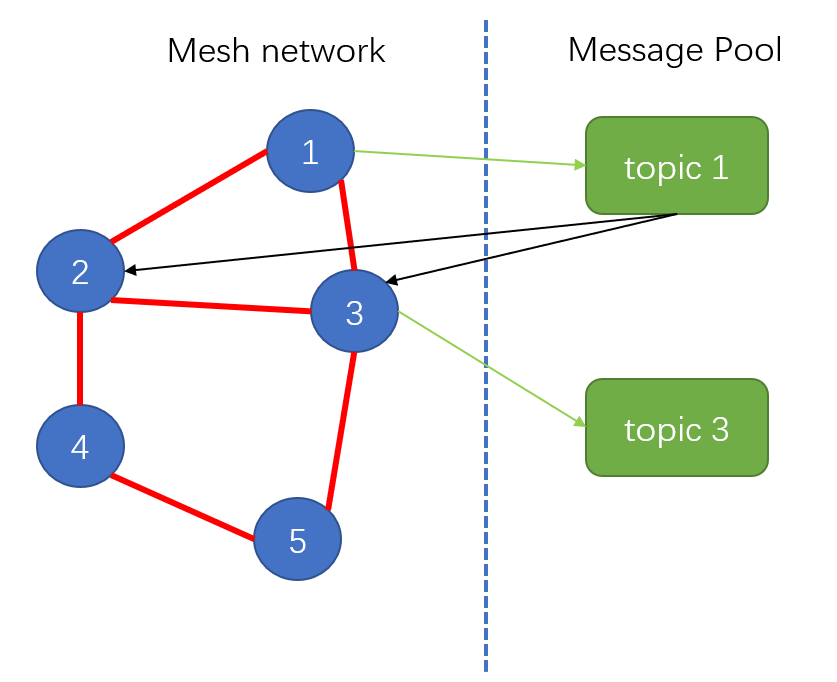
\includegraphics[width=1\textwidth]{pic/msg.png}
		  \end{figure}
		\end{columns}
	      \end{frame}

	      \begin{frame}{Experiment}
		We simulate the heat transfer process in a planar closed region:
		\begin{align*}
		  \frac{\partial u}{\partial t}=\alpha\Big(\frac{\partial^2u}{\partial x_1^2}+\frac{\partial^2u}{\partial x_2^2}\Big),
		\end{align*}
		with boundary conditions
		\begin{align*}
		  \frac{\partial u}{\partial x_1}\Big|_{t,0,x_2}=\frac{\partial u}{\partial x_1}\Big|_{t,l,x_2}=\frac{\partial u}{\partial x_2}\Big|_{t,x_1,0}=\frac{\partial u}{\partial x_2}\Big|_{t,x_1,l}=0.
		\end{align*}
		Sensors are randomly deployed in this region. With a grid and fixed sample frequency, the process can be discretized as:
		\begin{align*}
		  U(k+1)&=AU(k)+w(k)\\
		  Y(k)&=CU(k)+v(k).
		\end{align*}
	      \end{frame}

	      \begin{frame}{Experiment result}
		\begin{figure}[]
		  \centering
		  \includegraphics[width=0.65\textwidth]{pic/variance.pdf}
		  \caption{(a) Position and topology of $m$ sensors; (b) Centralized KF; (c) Local KF; (d) Our estimators in 10000 experiments.}
		\end{figure}
	      \end{frame}


	      \section{Conclusion}

	      \begin{frame}[standout]
		Thank you for your time! 
	      \end{frame}

	      \end{document}

